% =====================================================================
%  Ph.D. Thesis Proposal Defense — ~40 minutes
%  The Cost of Patient Autonomy in Cross-Silo Federated Learning
%
%  Compile:  latexmk -pdf proposal_defense.tex
%  Figures:  conda run -n thesis python make_figs.py   (run this first)
%
%  Timing target (~40 min talk + Q&A):
%     1. The Problem ................  5 min   (slides 3–9)
%     2. Thesis & RQs ..............  5 min   (slides 10–17)
%     3. Published Foundations .....  6 min   (slides 18–26)
%     4. System Design .............  5 min   (slides 27–34)
%     5. Executed: Utility Axis .... 10 min   (slides 35–48)
%     6. Model-Capacity Check ......  4 min   (slides 49–54)
%     7. Remaining Work ............  5 min   (slides 55–63)
%     8. Timeline / Limitations ....  3 min   (slides 64–69)
% =====================================================================
\documentclass[aspectratio=169, 11pt]{beamer}
\usetheme{metropolis}
\metroset{block=fill, progressbar=frametitle, numbering=fraction,
          sectionpage=progressbar, subsectionpage=none}

\definecolor{mCharcoal}{HTML}{2B2D33}
\definecolor{mCoral}{HTML}{E4572E}
\definecolor{mTeal}{HTML}{1B998B}
\definecolor{mGray}{HTML}{6B7280}
\definecolor{mLight}{HTML}{E5E7EB}
\setbeamercolor{frametitle}{bg=mCharcoal, fg=white}
\setbeamercolor{progress bar}{fg=mCoral}
\setbeamercolor{title separator}{fg=mCoral}
\setbeamercolor{alerted text}{fg=mCoral}
\setbeamercolor{example text}{fg=mTeal}
\setbeamercolor{block title alerted}{fg=white, bg=mCoral}
\setbeamercolor{block title example}{fg=white, bg=mTeal}
\setbeamercolor{normal text}{fg=mCharcoal, bg=white}
\setbeamertemplate{caption}{\raggedright\insertcaption\par}

\usepackage{booktabs}
\usepackage{graphicx}
\usepackage{tikz}
\usetikzlibrary{arrows.meta, positioning, fit, backgrounds, shapes.geometric}
\graphicspath{{figures/}{../Disertation_at_Work/}}

% compact helper for "status" tags
\newcommand{\done}{{\color{mTeal}\textbf{[EXECUTED]}}}
\newcommand{\planned}{{\color{mGray}\textbf{[PLANNED]}}}
% light variants for use on dark/coloured backgrounds (frame titles, filled
% block titles) where the coloured versions would vanish into the fill
\newcommand{\donelight}{{\color{white}\textbf{[EXECUTED]}}}
\newcommand{\plannedlight}{{\color{mLight}\textbf{[PLANNED]}}}
\newcommand{\hl}[1]{{\color{mCoral}\textbf{#1}}}

\title[The Cost of Patient Autonomy in Cross-Silo FL]%
      {The Cost of Patient Autonomy in\\Cross-Silo Federated Learning}
\subtitle{Ph.D.\ Thesis Proposal Defense}
\author{Thuan Nhan}
\institute{Ph.D.\ Program in Data Science}
\date{\today}

\begin{document}

\begin{frame}[plain]\titlepage\end{frame}

% ====================================================================
\begin{frame}{Roadmap of this talk}
\setbeamertemplate{section in toc}[sections numbered]
\begin{columns}[T]
\begin{column}{0.52\textwidth}
{\small\tableofcontents}
\end{column}
\begin{column}{0.46\textwidth}
\begin{block}{What I am asking for today}
Approval of a \textbf{measurement} thesis: one axis is already executed and
closed; the proposal is to build the second axis and join them.
\end{block}
\vspace{0.4em}
{\footnotesize
\textcolor{mTeal}{\textbf{Green}} marks results already in hand.\\
\textcolor{mGray}{\textbf{Gray}} marks proposed work.}
\end{column}
\end{columns}
\end{frame}

% ====================================================================
\section{The Problem}
% ====================================================================

\begin{frame}{Hospitals cannot pool patient data --- but need to}
\begin{columns}[T]
\begin{column}{0.56\textwidth}
\begin{itemize}
\item Clinical prediction models need \textbf{scale and diversity} to
      generalize across institutions.
\item Patient records cannot leave the hospital: HIPAA, GDPR, institutional
      liability, and genuine re-identification risk.
\item A single hospital's model \textbf{overfits its own case mix} --- it
      does not transfer.
\end{itemize}
\vspace{0.6em}
\begin{exampleblock}{Measured in this work}
Training on one silo alone (no federation) drops AUROC to
\textbf{0.616} on average, and as low as \textbf{0.516} --- barely better
than a coin flip --- versus \textbf{0.666} pooled.
\end{exampleblock}
\end{column}
\begin{column}{0.42\textwidth}
\centering
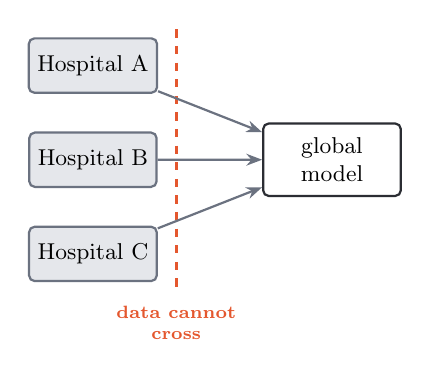
\begin{tikzpicture}[scale=0.92, transform shape,
  hosp/.style={draw=mGray, thick, rounded corners=2pt, fill=mLight,
               minimum width=1.7cm, minimum height=0.75cm, font=\small},
  wall/.style={draw=mCoral, very thick, dashed}]
  \node[hosp] (a) at (0,0)   {Hospital A};
  \node[hosp] (b) at (0,-1.3){Hospital B};
  \node[hosp] (c) at (0,-2.6){Hospital C};
  \draw[wall] (1.15,0.5) -- (1.15,-3.1);
  \node[font=\scriptsize\bfseries, text=mCoral, align=center]
       at (1.15,-3.55) {data cannot\\cross};
  \node[draw=mCharcoal, thick, rounded corners=2pt, minimum width=1.9cm,
        minimum height=1.0cm, font=\small, align=center]
       (m) at (3.3,-1.3) {global\\model};
  \foreach \n in {a,b,c}{\draw[-{Stealth[length=2mm]}, mGray, thick] (\n) -- (m);}
\end{tikzpicture}
\end{column}
\end{columns}
\end{frame}

% --------------------------------------------------------------------
\begin{frame}{Federated learning is the standard answer}
\begin{itemize}
\item Each hospital trains \textbf{locally}; only model weights are shared.
\item A coordinator averages the weights (\textbf{FedAvg}, McMahan 2017) and
      broadcasts the new global model.
\item Raw records never move. Repeat for $R$ rounds.
\end{itemize}
\vspace{0.5em}
\begin{center}
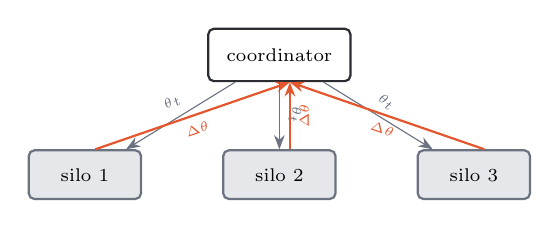
\begin{tikzpicture}[scale=0.95, transform shape,
  b/.style={draw=mGray, thick, rounded corners=2pt, fill=mLight,
            minimum width=1.5cm, minimum height=0.65cm, font=\scriptsize},
  s/.style={draw=mCharcoal, thick, rounded corners=2pt,
            minimum width=1.9cm, minimum height=0.7cm, font=\scriptsize}]
  \node[s] (srv) at (0,0) {coordinator};
  \node[b] (s1) at (-2.6,-1.6) {silo 1};
  \node[b] (s2) at (0,-1.6)    {silo 2};
  \node[b] (s3) at (2.6,-1.6)  {silo 3};
  \foreach \n in {s1,s2,s3}{
    \draw[-{Stealth[length=1.8mm]}, mGray] (srv) -- node[font=\tiny, sloped,
      above, text=mGray] {$\theta_t$} (\n);
    \draw[-{Stealth[length=1.8mm]}, mCoral, thick] ([xshift=4pt]\n.north) --
      node[font=\tiny, sloped, below, text=mCoral] {$\Delta\theta$}
      ([xshift=4pt]srv.south);}
\end{tikzpicture}
\end{center}
\vspace{0.3em}
{\footnotesize FedAvg's well-known weakness --- sensitivity to non-IID data ---
turns out to be exactly what makes this thesis measurable. More on that later.}
\end{frame}

% --------------------------------------------------------------------
\begin{frame}{But federation alone does not give patients control}
\begin{itemize}
\item FL keeps data \emph{inside} the hospital. It says nothing about whether
      \textbf{the patient} agreed to be in the model.
\item Consent today is a paper form: coarse, one-time, effectively
      irrevocable once training has happened.
\item GDPR Art.~17 (``right to erasure'') and emerging U.S.\ rules point the
      other way: consent should be \textbf{fine-grained, dynamic, revocable}.
\end{itemize}
\vspace{0.5em}
\begin{alertblock}{The literature's move}
A growing body of work adds a \textbf{blockchain consent layer}: smart
contracts record grant/revoke, so a patient can withdraw at any time and the
next training round must respect it.
\end{alertblock}
\end{frame}

% --------------------------------------------------------------------
\begin{frame}{The gap: everyone builds it, nobody prices it}
\begin{columns}[T]
\begin{column}{0.55\textwidth}
The consent-on-blockchain literature is \textbf{overwhelmingly
architectural}:
\begin{itemize}
\item ``We designed a system where patients can revoke consent.''
\item ``Here is the contract, here is the workflow.''
\item Evaluation stops at \emph{feasibility} --- it compiles, it runs,
      gas is reported for a toy workload.
\end{itemize}
\vspace{0.4em}
Patient autonomy is treated as an \textbf{unqualified good}: a feature to be
added, never a cost to be measured.
\end{column}
\begin{column}{0.43\textwidth}
\begin{alertblock}{What is missing}
Nobody has asked:
\begin{enumerate}
\item What does consent governance \textbf{cost per training round}?
\item What does revocation do to \textbf{model accuracy}?
\item Where do those two costs make the system \textbf{stop working}?
\end{enumerate}
\end{alertblock}
\end{column}
\end{columns}
\end{frame}

% --------------------------------------------------------------------
\begin{frame}{Why the question is not rhetorical}
Revocable consent breaks an assumption every FL algorithm makes.
\vspace{0.6em}
\begin{columns}[T]
\begin{column}{0.48\textwidth}
\begin{block}{Standard FL assumes}
A \textbf{fixed} client population and a \textbf{stationary} data
distribution across rounds. Convergence guarantees are stated in those terms.
\end{block}
\end{column}
\begin{column}{0.48\textwidth}
\begin{alertblock}{Consent-gated FL delivers}
A population that \textbf{changes every round}, in a direction that is
\emph{not} random --- patients who withdraw are correlated with their
diagnosis, their hospital, their outcome.
\end{alertblock}
\end{column}
\end{columns}
\vspace{0.7em}
\begin{itemize}
\item Every revocation is also an \textbf{on-chain transaction} --- gas,
      latency, and a consent-set resolution the coordinator must perform
      before it can start the round.
\item So autonomy is paid for \textbf{twice}: once in systems overhead, once
      in model utility.
\end{itemize}
\end{frame}

% --------------------------------------------------------------------
\begin{frame}{The reframe}
\begin{center}
\Large
Patient autonomy is not a feature to be built.\\[0.5em]
It is a \hl{cost to be measured}.
\end{center}
\vspace{1.0em}
\begin{columns}[T]
\begin{column}{0.48\textwidth}
\begin{block}{The field's framing}
``Can we give patients revocable consent in federated healthcare ML?''\\[0.3em]
{\footnotesize Answer: yes, obviously --- and it has been answered many times.}
\end{block}
\end{column}
\begin{column}{0.48\textwidth}
\begin{exampleblock}{This thesis's framing}
``\textbf{What does it cost}, and \textbf{where does it break}?''\\[0.3em]
{\footnotesize Answer: a two-axis measurement and a frontier with explicit
breaking points.}
\end{exampleblock}
\end{column}
\end{columns}
\end{frame}

% --------------------------------------------------------------------
\begin{frame}{The two axes of cost}
\begin{columns}[T]
\begin{column}{0.49\textwidth}
\begin{block}{Axis 1 --- Systems cost \quad\planned}
On-chain governance overhead added to \emph{every} round:
\begin{itemize}\small
\item consent-set resolution
\item grant/revoke transactions (gas)
\item encrypted-record retrieval
\item latency, bandwidth
\end{itemize}
\end{block}
\end{column}
\begin{column}{0.49\textwidth}
\begin{block}{Axis 2 --- Utility cost \quad\done}
Accuracy lost because revocable consent makes the training population
\textbf{non-stationary}:
\begin{itemize}\small
\item who withdraws, and when
\item whether withdrawal shifts the distribution
\item whether a whole institution exits
\end{itemize}
\end{block}
\end{column}
\end{columns}
\vspace{0.6em}
\begin{alertblock}{The deliverable}
Not two separate numbers --- a \textbf{joint cost--utility frontier}, swept
over the same consent knobs, with the breaking points marked on it.
\end{alertblock}
\end{frame}

% --------------------------------------------------------------------
\begin{frame}{What a frontier buys you that a feature list does not}
\begin{center}
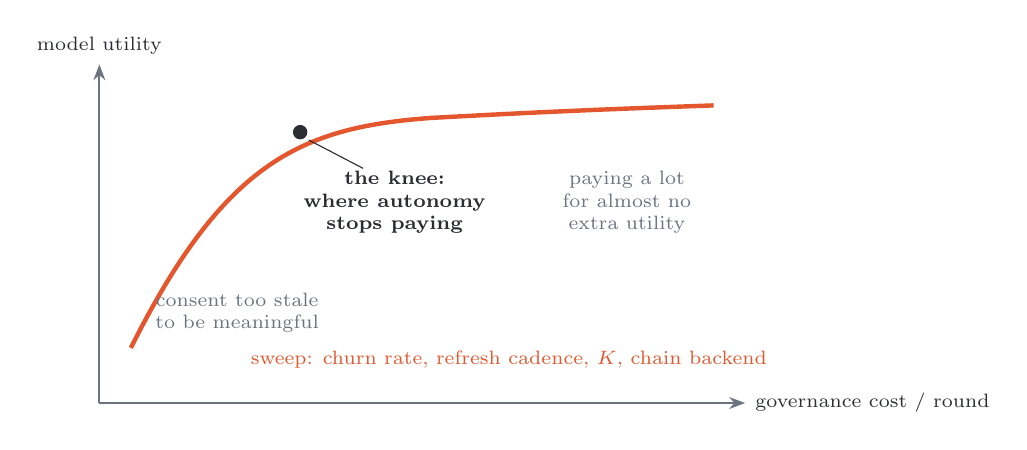
\begin{tikzpicture}[scale=1.0]
  \draw[-{Stealth[length=2mm]}, mGray, thick] (0,0) -- (8.2,0)
        node[right, font=\scriptsize, text=mCharcoal] {governance cost / round};
  \draw[-{Stealth[length=2mm]}, mGray, thick] (0,0) -- (0,4.3)
        node[above, font=\scriptsize, text=mCharcoal] {model utility};
  % knee curve
  \draw[mCoral, ultra thick]
    (0.4,0.7) .. controls (1.6,3.1) and (2.6,3.5) .. (4.2,3.62)
              .. controls (6.0,3.72) and (7.0,3.75) .. (7.8,3.78);
  % knee marker
  \fill[mCharcoal] (2.55,3.44) circle (2.6pt);
  \node[font=\scriptsize\bfseries, text=mCharcoal, align=center]
       at (3.75,2.55) {the knee:\\where autonomy\\stops paying};
  \draw[mCharcoal, thin] (2.66,3.34) -- (3.35,2.98);
  % regions
  \node[font=\scriptsize, text=mGray, align=center] at (1.75,1.15)
       {consent too stale\\to be meaningful};
  \node[font=\scriptsize, text=mGray, align=center] at (6.7,2.55)
       {paying a lot\\for almost no\\extra utility};
  \node[font=\scriptsize, text=mCoral] at (5.2,0.55)
       {sweep: churn rate, refresh cadence, $K$, chain backend};
\end{tikzpicture}
\end{center}
\vspace{-0.2em}
{\footnotesize A frontier tells a hospital consortium \emph{which operating
point to pick}. ``We support revocation'' does not. \hfill\textcolor{mGray}{(H3
--- shape is hypothesized, not yet measured.)}}
\end{frame}

% ====================================================================
\section{Thesis Statement and Research Questions}
% ====================================================================

\begin{frame}{Thesis statement}
\begin{alertblock}{Thesis}
This dissertation \textbf{quantifies the two-axis cost of patient
autonomy} --- governance overhead and model-utility degradation --- in a
consent-gated cross-silo federated healthcare system, and identifies the
configurations and \textbf{breaking points} at which patient-controlled
federated clinical prediction remains practical.
\end{alertblock}
\vspace{0.7em}
\begin{columns}[T]
\begin{column}{0.48\textwidth}
\begin{exampleblock}{This is}
A \textbf{measurement and systems} contribution. The artifacts are
cost--utility curves and the breaking points on them.
\end{exampleblock}
\end{column}
\begin{column}{0.48\textwidth}
\begin{block}{This is not}
A new FL algorithm. A peak-accuracy result. A blockchain system paper ---
that component is already published.
\end{block}
\end{column}
\end{columns}
\end{frame}

% --------------------------------------------------------------------
\begin{frame}{A standard I hold myself to}
\begin{center}
\large
The evaluation must surface a \hl{non-obvious} finding.
\end{center}
\vspace{0.8em}
\begin{columns}[T]
\begin{column}{0.47\textwidth}
\begin{block}{Would not count}
``More dropout lowers accuracy.''\\[0.4em]
{\footnotesize True, trivial, and predictable without running anything.
A thesis that only establishes this has measured nothing.}
\end{block}
\end{column}
\begin{column}{0.47\textwidth}
\begin{exampleblock}{Would count --- and does}
``\textbf{Who} leaves matters more than \textbf{how many} leave.''\\[0.4em]
{\footnotesize Overturns the headcount intuition, and changes what a
consortium should actually worry about. \done}
\end{exampleblock}
\end{column}
\end{columns}
\vspace{0.6em}
{\footnotesize Each research question below carries an explicit
non-obvious-finding target, not just a hypothesis.}
\end{frame}

% --------------------------------------------------------------------
\begin{frame}{RQ1 --- The systems-cost axis \hfill \plannedlight}
\begin{block}{Question}
How does on-chain consent-governance overhead scale with \textbf{churn rate},
\textbf{consent-refresh cadence}, \textbf{federation size $K$}, and
\textbf{chain backend} (local / permissioned / public)?
\end{block}
\begin{alertblock}{H1}
Per-round governance cost is dominated by \textbf{consent-set resolution} and
grows with churn rate, crossing a \textbf{backend-dependent threshold} beyond
which per-round enforcement is infeasible and consent must be
\textbf{amortized} across rounds.
\end{alertblock}
\begin{exampleblock}{Non-obvious target}
Locate that threshold, and characterize the
\textbf{amortization--staleness tradeoff} it forces: amortizing consent
means training on consent state that is knowingly out of date.
\end{exampleblock}
\end{frame}

% --------------------------------------------------------------------
\begin{frame}{RQ2 --- The utility-cost axis \hfill \donelight}
\begin{block}{Question}
How does model utility degrade as a function of consent dynamics, and do
\textbf{physically distinct churn regimes} degrade it differently?
\end{block}
\vspace{-0.2em}
\begin{alertblock}{H2}
The regimes are \textbf{not interchangeable}: transient churn is near-harmless
because contributions re-enter, whereas whole-silo departure inflicts a
non-IID shock that \textbf{dominates all per-patient effects}.
\end{alertblock}
\vspace{-0.2em}
\begin{exampleblock}{Non-obvious target --- \textbf{confirmed}}
Show that \emph{who} leaves matters more than \emph{how many} leave,
overturning the headcount model. Confirmed by a count-matched isolation test
over five seeds, and shown \textbf{model-independent} by a full rerun with a
higher-capacity client.
\end{exampleblock}
\end{frame}

% --------------------------------------------------------------------
\begin{frame}{RQ3 --- The joint frontier \hfill \plannedlight}
\begin{block}{Question}
Where is the joint cost--utility frontier, and what configurations keep the
system in a \textbf{practical operating region}?
\end{block}
\begin{alertblock}{H3}
There exist consent-refresh cadences that recover \textbf{most of the utility}
of per-round enforcement at \textbf{a fraction of the governance cost} ---
i.e.\ the frontier is sharply \textbf{knee-shaped}, not linear.
\end{alertblock}
\begin{exampleblock}{Non-obvious target}
Identify the knee and the deployment regimes it implies. If the frontier is
knee-shaped, ``refresh consent every round'' --- which every system paper
assumes --- is the \emph{wrong} default.
\end{exampleblock}
\end{frame}

% --------------------------------------------------------------------
\begin{frame}{RQ4 --- Multi-project consent \hfill \plannedlight}
\begin{block}{Question}
Can a \textbf{single consent layer} govern patients enrolled in several
federated studies at once (a patient\,$\times$\,study matrix), and what is the
\textbf{marginal governance cost} per additional study?
\end{block}
\begin{alertblock}{H4}
Multi-project consent adds \textbf{bounded, sub-linear} on-chain overhead,
because consent state is \textbf{shared infrastructure} rather than
per-study duplication.
\end{alertblock}
\begin{exampleblock}{Non-obvious target}
Demonstrate the framework generalizes beyond a single disease model
\textbf{without building a second one} --- the marginal cost, not a second
end-to-end system, is the evidence.
\end{exampleblock}
\end{frame}

% --------------------------------------------------------------------
\begin{frame}{Contributions}
\scriptsize
\begin{enumerate}\setlength\itemsep{0.5em}
\item[\textbf{C1}] \textbf{A dual-axis measurement of the cost of patient
  autonomy.} First joint characterization of governance overhead and utility
  degradation under revocable consent, as cost--utility curves with explicit
  breaking points. \hfill{\scriptsize(RQ1, RQ3)}
\item[\textbf{C2}] \textbf{A three-regime model of consent churn.} Separates
  transient departure, permanent withdrawal, and whole-silo exit into
  physically distinct regimes; confirms \emph{who} $>$ \emph{how many} via a
  count-matched isolation test; shows it is model-independent.
  \hfill{\scriptsize(RQ2) \done}
\item[\textbf{C3}] \textbf{A multi-project consent framework.} A
  patient\,$\times$\,study consent matrix at the contract level, with measured
  marginal cost per study. \hfill{\scriptsize(RQ4)}
\item[\textbf{C4}] \textbf{Validated, reusable components and methodology.}
  A scalable multimodal classifier; a patient-controlled blockchain/IPFS
  consent layer with a \textbf{validated on-chain cost-measurement
  methodology}; a multi-institutional regime-shift analysis.
  \hfill{\scriptsize(feasibility) \done}
\item[\textbf{C5}] \textbf{An open, reproducible testbed and benchmark.}
  Testbed, contracts, churn-schedule generators, and Synthea-derived
  populations, released open-source. \hfill{\scriptsize(all RQs)}
\end{enumerate}
\end{frame}

% --------------------------------------------------------------------
\begin{frame}{Scope: what is deliberately in and out}
\small
\begin{columns}[T]
\begin{column}{0.49\textwidth}
\begin{exampleblock}{In scope}
\begin{itemize}\small
\item Simulated cross-silo consortium, $K{=}3$ and small $K$
\item 30-day readmission on Diabetes 130 (real, 102k encounters)
\item Class-weighted FedAvg as the reference instrument
\item Consent \textbf{governance} and \textbf{data autonomy}
\item Gas/latency across local, permissioned, public backends
\end{itemize}
\end{exampleblock}
\end{column}
\begin{column}{0.49\textwidth}
\begin{block}{Out of scope}
\begin{itemize}\small
\item Live multi-hospital deployment
\item Daily EHR transaction processing, billing workflows
\item Supply-chain forecasting as a co-equal target
\item \textbf{Formal privacy guarantees} in Year 1 --- see next slide
\item Peak accuracy on the clinical task
\end{itemize}
\end{block}
\end{column}
\end{columns}
\end{frame}

% --------------------------------------------------------------------
\begin{frame}{One honesty commitment I want on the record}
\begin{alertblock}{The Year-1 claim is \emph{consent governance and data
autonomy} --- not \emph{privacy}}
FedAvg alone provides \textbf{leaky data-locality}, not a differential-privacy
guarantee. Gradients leak. Calling this system ``privacy-preserving'' would be
overclaiming, and I do not.
\end{alertblock}
\vspace{0.6em}
\begin{itemize}
\item Differential privacy (DP-SGD) and secure aggregation are
      \textbf{composable layers} added in a later thrust.
\item That thrust \emph{earns} the word ``privacy'' --- and adds a
      \textbf{third axis} (noise $\rightarrow$ accuracy loss) to the same
      frontier.
\item Deferring it is a scoping decision, not an oversight: the two axes must
      be measured cleanly before a third is layered on.
\end{itemize}
\end{frame}

% ====================================================================
\section{Foundations: Three Published Components}
% ====================================================================

\begin{frame}{The proposal does not start from zero}
Three published papers supply the instruments this thesis needs.
\vspace{0.3em}
\begin{center}\scriptsize
\begin{tabular}{p{3.3cm}p{4.1cm}p{4.6cm}}
\toprule
\textbf{Published work} & \textbf{What it built} & \textbf{What it gives the thesis}\\
\midrule
Spark benchmarking\newline (cervical cancer) &
Scalable Spark/SparkML pipeline vs.\ scikit-learn and a CNN &
The \textbf{compute-placement rule}, and the Year-3 image baseline\\
\addlinespace
Patient-centric\newline blockchain EHR &
Ethereum + IPFS consent layer with grant/revoke &
The \textbf{consent layer} and a \textbf{validated on-chain cost methodology}
--- the RQ1 instrument\\
\addlinespace
Supply-chain\newline regime shift (COVID) &
Lead-time models across a multi-institutional supply chain &
Documented \textbf{cross-institution regime shift} --- the real-world cousin
of non-IID shock\\
\bottomrule
\end{tabular}
\end{center}
\vspace{0.4em}
{\footnotesize These are \emph{feasibility and instrumentation}, not the
thesis contribution itself.}
\end{frame}

% --------------------------------------------------------------------
\begin{frame}{Component 1 --- Spark benchmarking (published)}
\begin{columns}[T]
\begin{column}{0.55\textwidth}
\textbf{What was built.} A scalable cervical-cancer detection pipeline on
Apache Spark/SparkML, benchmarked against scikit-learn and a CNN across
\textbf{two modalities}.
\vspace{0.5em}
\begin{itemize}\small
\item \textbf{Tabular} (cervical risk factors): Spark Random Forest reached
      \textbf{0.96} accuracy (0.99 precision, 0.97 recall) after ADASYN
      balancing of a strongly imbalanced cohort.
\item \textbf{Scalability}: scaling data $0.27 \rightarrow 217$\,MB, Spark
      crossed over to $\approx$\,\textbf{3.3$\times$ faster} than
      scikit-learn as volume grew.
\item \textbf{Images} (SipakMed Pap smears): a CNN reached
      \textbf{92.75\%} where Spark's general classifiers plateaued near
      \textbf{73\%}.
\end{itemize}
\end{column}
\begin{column}{0.43\textwidth}
\centering
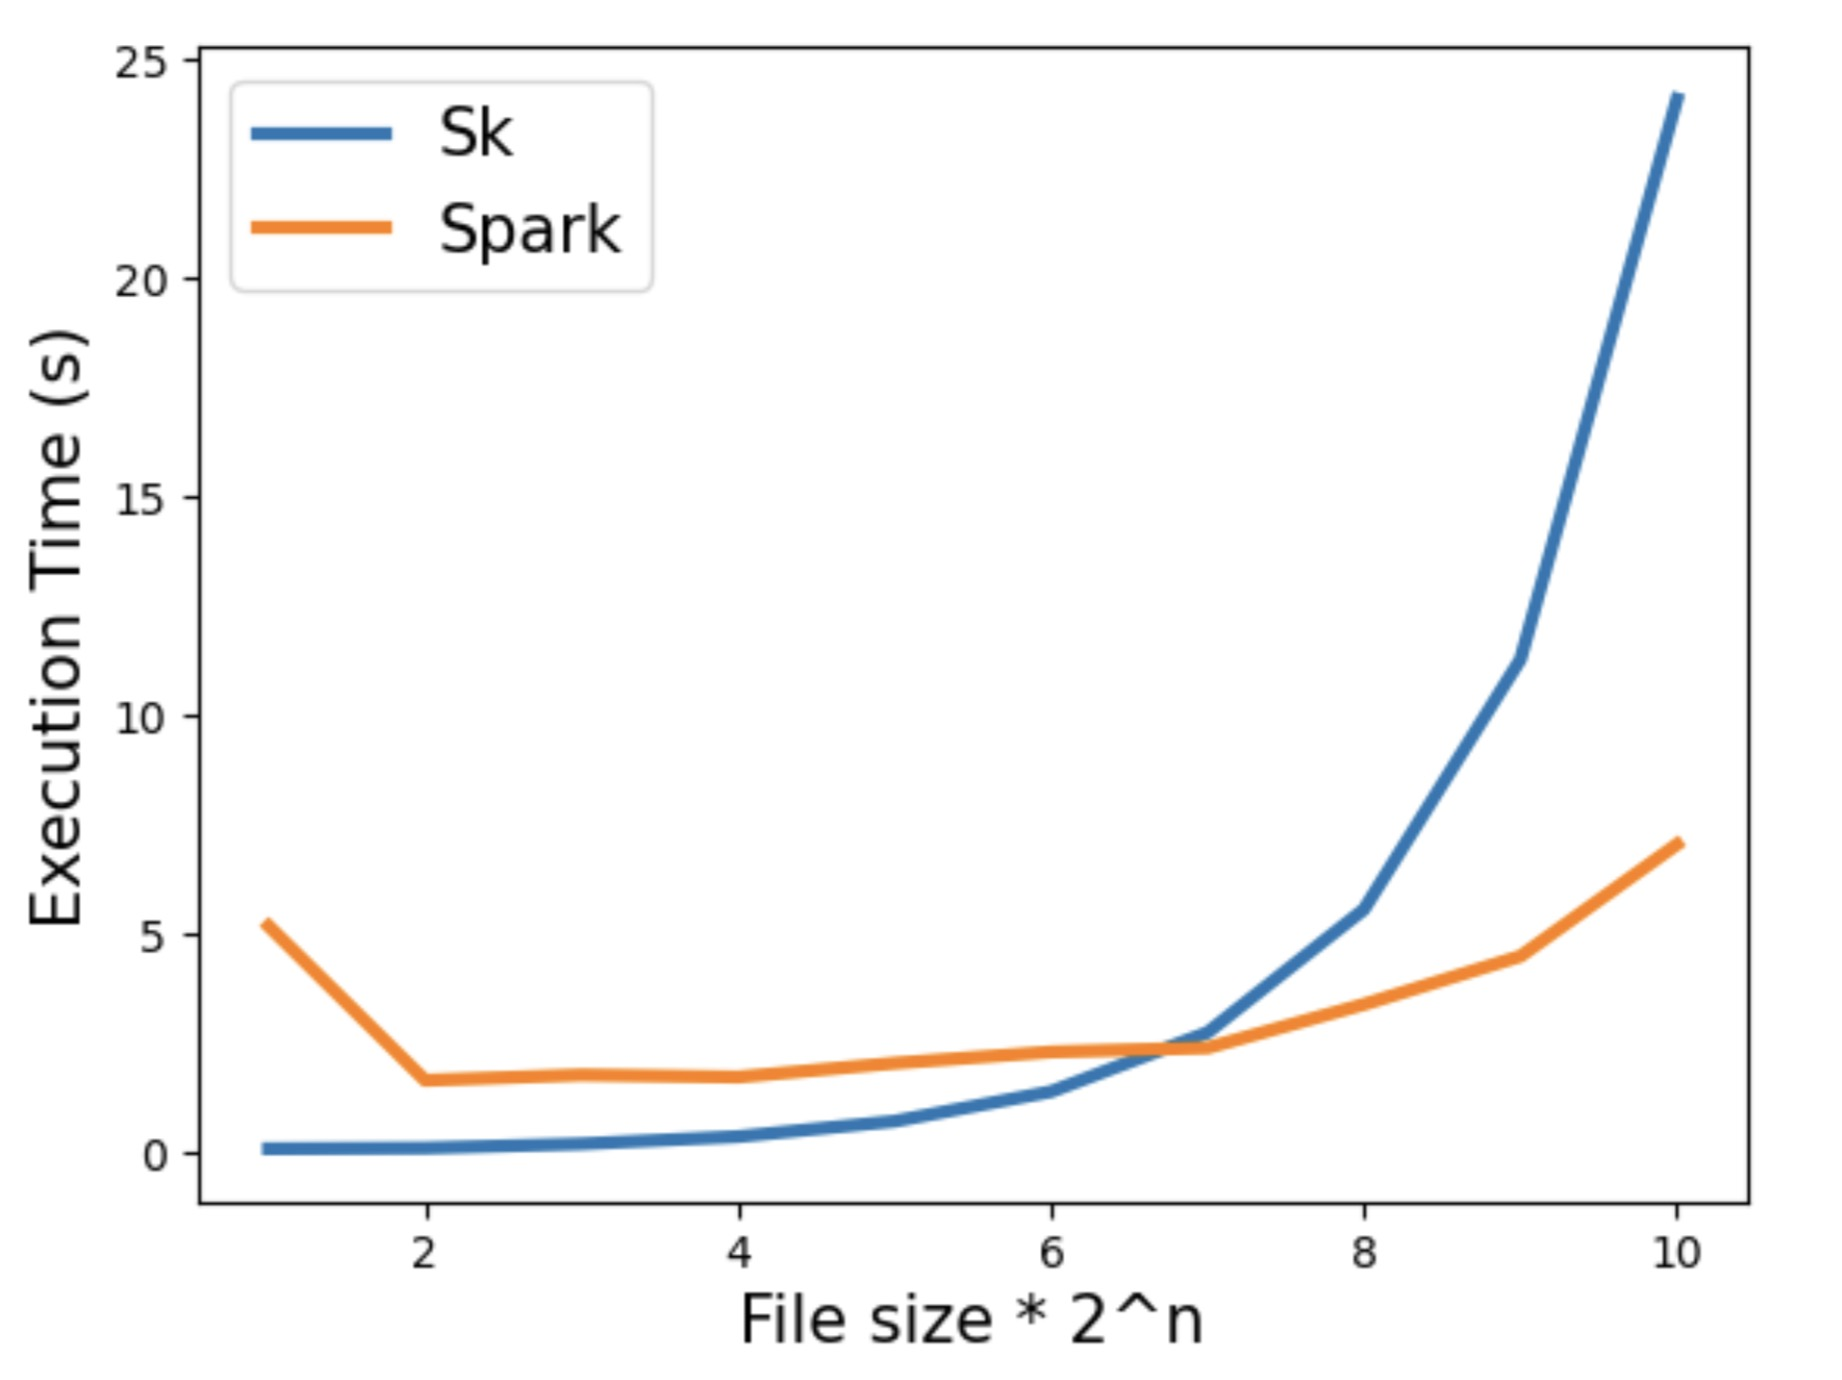
\includegraphics[width=\linewidth]{SparkPaperFigure/Scale-Sk-Spark.jpg}\\
{\scriptsize Spark vs.\ scikit-learn as data volume grows.}
\end{column}
\end{columns}
\end{frame}

% --------------------------------------------------------------------
\begin{frame}{Component 1 --- what it gives the thesis}
\begin{exampleblock}{The compute-placement rule (empirically grounded)}
Distributed / Spark compute \textbf{earns its place on large image data} but
is \textbf{overkill on small tabular data}.
\end{exampleblock}
\vspace{0.7em}
\begin{itemize}
\item This rule is \textbf{honored, not ignored}, in the thesis plan:
      Year 1 uses \textbf{plain tabular federated training}; Spark and images
      are deferred to Year 3.
\item Without it, the obvious --- and wrong --- move would be to put the
      federated readmission task on Spark because it sounds more impressive.
\item It also supplies the \textbf{Year-3 image task and baseline}, so the
      image extension does not start cold.
\end{itemize}
\vspace{0.4em}
{\footnotesize A negative-space contribution: prior work telling me what
\emph{not} to build.}
\end{frame}

% --------------------------------------------------------------------
\begin{frame}{Component 2 --- Patient-centric blockchain EHR (published)}
\begin{columns}[T]
\begin{column}{0.54\textwidth}
A Python application mediates an \textbf{Ethereum smart contract} and
\textbf{IPFS} storage.
\begin{itemize}\scriptsize
\item Records encrypted (Fernet), stored \textbf{off-chain on IPFS}.
\item The contract holds only: content identifier, owner wallet,
      authorized-viewer list, key.
\item Exposes \texttt{grantPermission}, \texttt{rescindPermission},
      \texttt{viewInformation}, \texttt{isViewerAuthorized}.
\end{itemize}
\vspace{0.3em}
\begin{alertblock}{Design invariant}
\small\textbf{No clinical data on the ledger.} An immutable, replicated chain
holding PHI would be a privacy liability, not a feature.
\end{alertblock}
\end{column}
\begin{column}{0.44\textwidth}
\centering
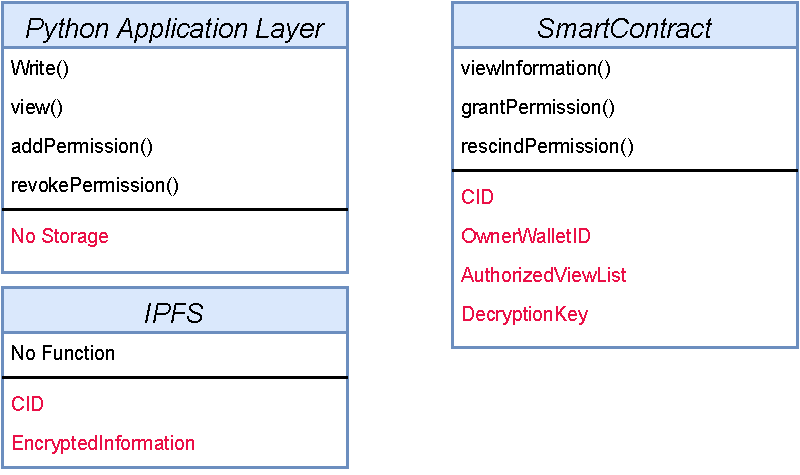
\includegraphics[width=\linewidth]{BlockChainPaper/ComponentOverview.pdf}\\
{\scriptsize System component overview.}
\end{column}
\end{columns}
\end{frame}

% --------------------------------------------------------------------
\begin{frame}{Component 2 --- measured cost on a local chain}
\begin{columns}[T]
\begin{column}{0.5\textwidth}
\textbf{Ganache} (single-node local chain):
\vspace{0.4em}
\begin{center}\small
\begin{tabular}{lrr}
\toprule
Operation & Time (s) & Cost (ETH)\\
\midrule
Add permission    & 0.0521 & 0.00099\\
Revoke permission & 0.0705 & 0.00119\\
\bottomrule
\end{tabular}
\end{center}
\vspace{0.5em}
\begin{itemize}\small
\item All operations under \textbf{0.1\,s}; IPFS retrieval typically under
      \textbf{0.3\,s}.
\item \textbf{Revoke costs more than add} --- consistently, on both backends.
\item Ganache variance is near zero --- but it is \emph{one node}, so this is
      a best case, not a deployment estimate.
\end{itemize}
\end{column}
\begin{column}{0.48\textwidth}
\centering
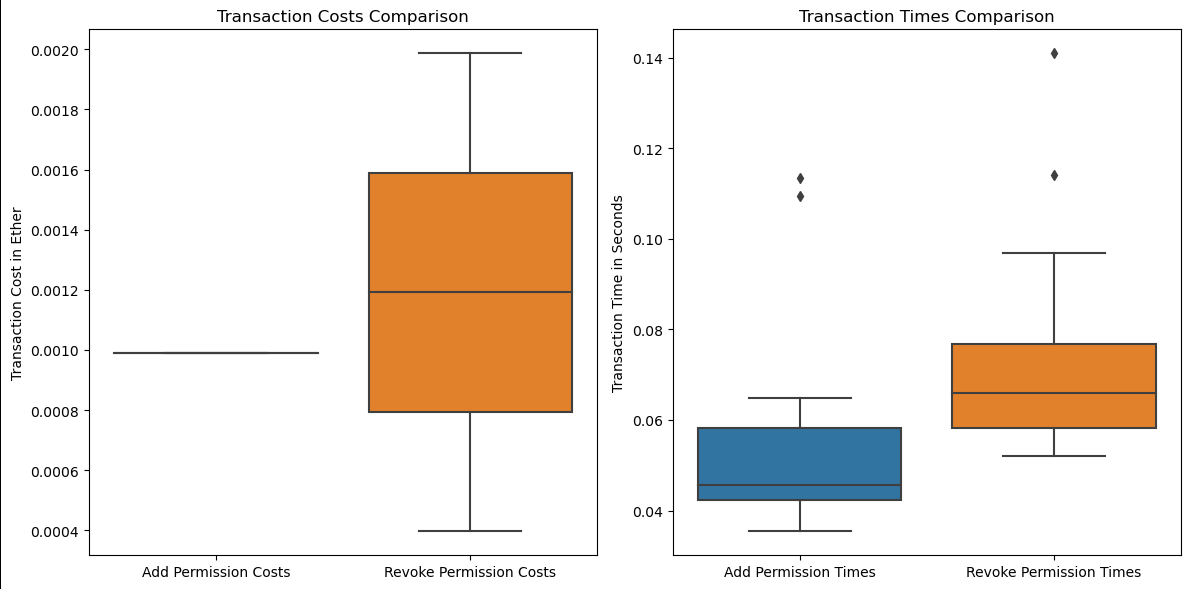
\includegraphics[width=0.95\linewidth]{BlockChainPaper/GanacheBoxPlot.png}\\
{\scriptsize Ganache transaction cost/time distributions.}
\end{column}
\end{columns}
\end{frame}

% --------------------------------------------------------------------
\begin{frame}{Component 2 --- and on a public chain, it falls apart}
\begin{columns}[T]
\begin{column}{0.52\textwidth}
\textbf{Sepolia} (public testnet), measured across the day:
\begin{itemize}\small
\item Fastest: add \textbf{8.84\,s}, revoke \textbf{12.01\,s}.
\item Peaks: revoke \textbf{107.99\,s} at 1\,AM; add \textbf{55.09\,s} at
      12\,PM.
\item Congestion 6--9\,AM CT caused outright \textbf{transaction failures}
      under our wallet settings.
\item Revoke cost peaked at \textbf{0.0198 ETH} --- roughly $20\times$ the
      Ganache figure.
\end{itemize}
\vspace{0.2em}
\begin{alertblock}{Why this matters for RQ1}
\small Latency is \textbf{heavy-tailed}, not Gaussian. A mean would hide the
failures --- so RQ1 reports \textbf{distributions}.
\end{alertblock}
\end{column}
\begin{column}{0.46\textwidth}
\centering
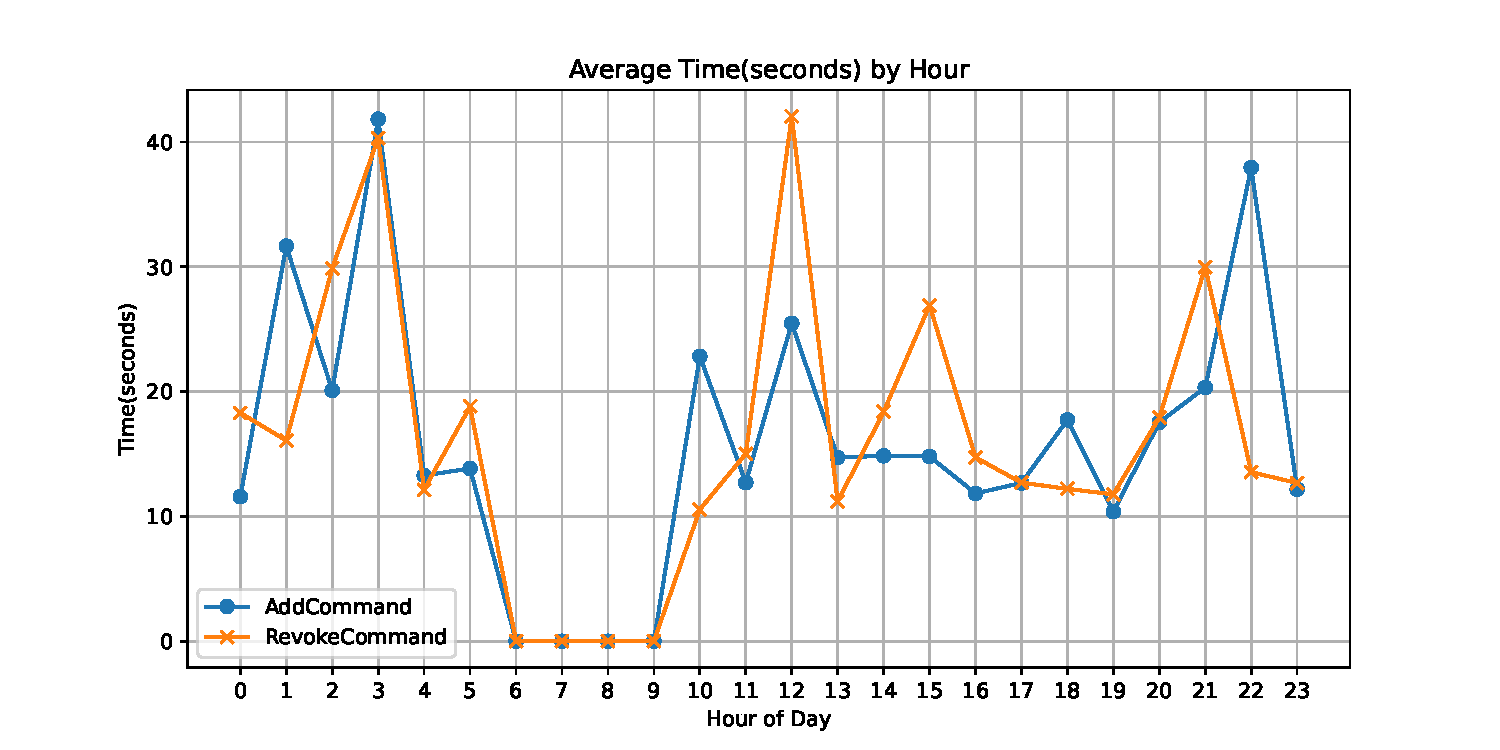
\includegraphics[width=\linewidth]{BlockChainPaper/Sepholia_transaction_time_plots.pdf}\\
{\scriptsize Sepolia transaction time through the day.}
\end{column}
\end{columns}
\end{frame}

% --------------------------------------------------------------------
\begin{frame}{Component 2 --- what it gives the thesis}
\begin{exampleblock}{The RQ1 instrument}
A \textbf{validated methodology for measuring on-chain governance cost} ---
latency and gas per operation, across backends, reported as distributions.
\end{exampleblock}
\vspace{0.6em}
\begin{itemize}
\item The consent-layer \textbf{design and grant/revoke semantics} carry over
      directly.
\item The 4-orders-of-magnitude spread between Ganache (0.05\,s) and congested
      Sepolia (108\,s) is \textbf{precisely the H1 threshold question}: at what
      churn rate does per-round consent enforcement stop keeping up?
\item The published paper's own stated future work --- ``extensive load
      testing is necessary'' --- is \textbf{exactly what RQ1 does}.
\end{itemize}
\end{frame}

% --------------------------------------------------------------------
\begin{frame}{Component 3 --- Supply-chain regime shift (published)}
\begin{columns}[T]
\begin{column}{0.53\textwidth}
Lead-time modeling across a large multi-institutional healthcare supply chain.
\begin{itemize}\small
\item Random Forest regression, \textbf{$R^2 \geq 0.87$}.
\item \textbf{Feature importance shifts} between normal operation and crisis
      (pandemic) operation --- the same model, the same institutions,
      different drivers.
\end{itemize}
\vspace{0.3em}
\begin{exampleblock}{What it gives the thesis}
\small A \textbf{documented, real-world multi-institution regime shift} ---
the empirical cousin of the non-IID shock studied in RQ2. Cross-institution
distribution shift is not a simulation artifact.
\end{exampleblock}
\end{column}
\begin{column}{0.45\textwidth}
\centering
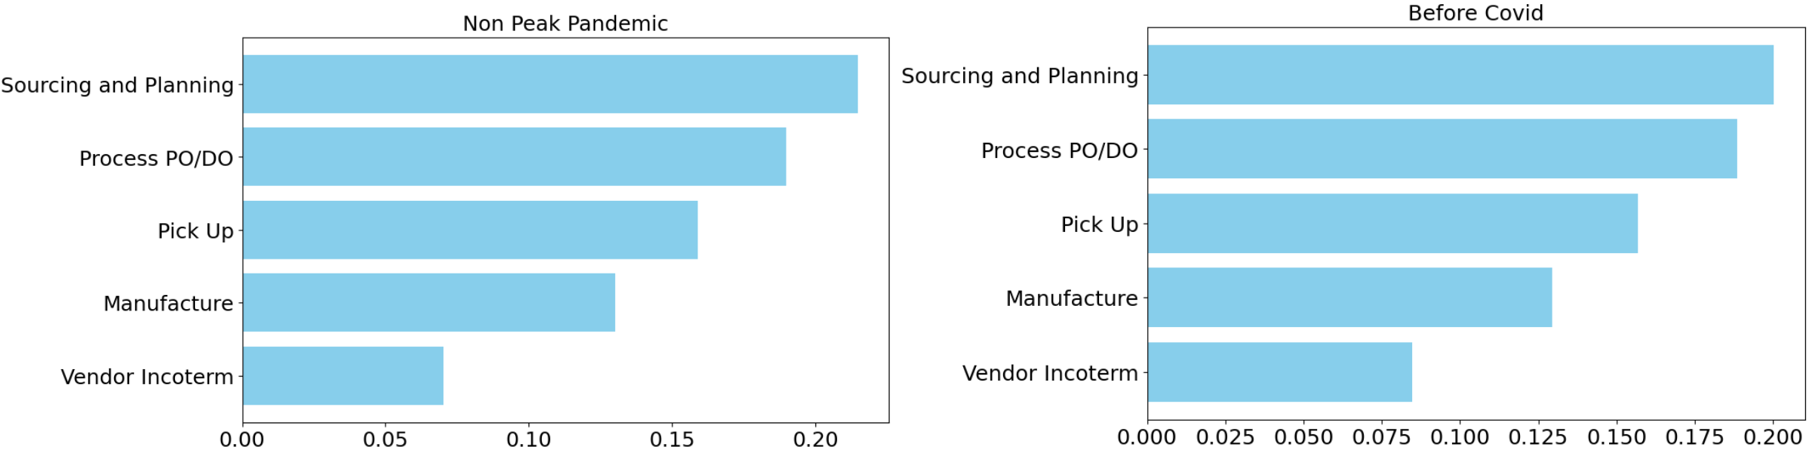
\includegraphics[width=0.92\linewidth]{CovidPaper/NormalOperation.png}\\[0.3em]
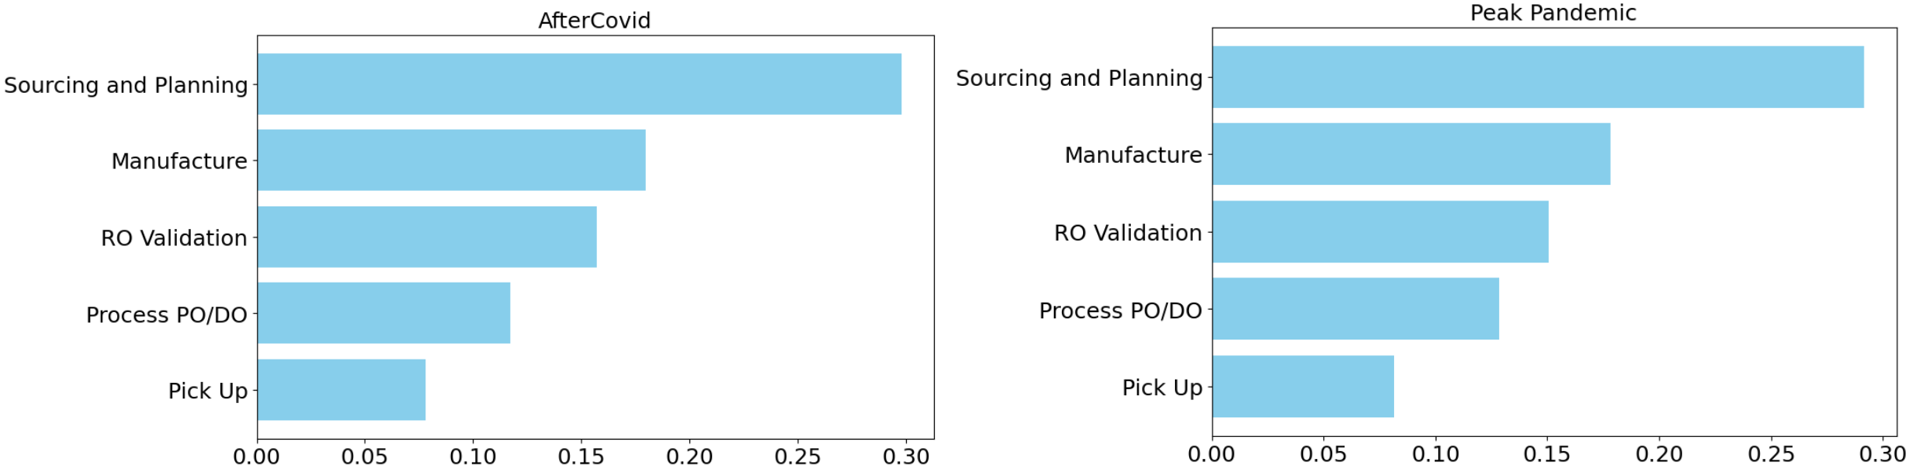
\includegraphics[width=0.92\linewidth]{CovidPaper/StressOperation.png}\\
{\scriptsize Normal vs.\ stressed operating regimes.}
\end{column}
\end{columns}
\end{frame}

% ====================================================================
\section{System Design}
% ====================================================================

\begin{frame}{Consent-gated cross-silo FL: the architecture}
\begin{center}
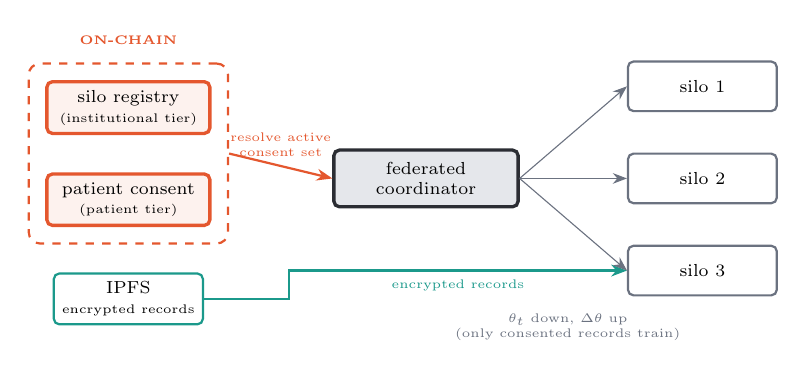
\begin{tikzpicture}[scale=0.9, transform shape,
  box/.style={draw=mGray, thick, rounded corners=2pt, fill=white,
              minimum width=2.1cm, minimum height=0.7cm, font=\scriptsize,
              align=center},
  chain/.style={draw=mCoral, very thick, rounded corners=2pt, fill=mCoral!8,
              minimum width=2.3cm, minimum height=0.7cm, font=\scriptsize,
              align=center},
  srv/.style={draw=mCharcoal, very thick, rounded corners=2pt, fill=mLight,
              minimum width=2.6cm, minimum height=0.8cm, font=\scriptsize,
              align=center}]

  \node[chain] (reg)  at (-4.2, 1.6) {silo registry\\{\tiny(institutional tier)}};
  \node[chain] (cons) at (-4.2, 0.3) {patient consent\\{\tiny(patient tier)}};
  \node[box, draw=mTeal]   (ipfs) at (-4.2,-1.1) {IPFS\\{\tiny encrypted records}};
  \begin{scope}[on background layer]
    \node[draw=mCoral, dashed, thick, rounded corners=4pt,
          fit=(reg)(cons), inner sep=6pt] (chainbox) {};
  \end{scope}
  \node[font=\tiny\bfseries, text=mCoral] at (-4.2,2.55) {ON-CHAIN};

  \node[srv] (coord) at (0,0.6) {federated\\coordinator};
  \node[box] (s1) at (3.9, 1.9) {silo 1};
  \node[box] (s2) at (3.9, 0.6) {silo 2};
  \node[box] (s3) at (3.9,-0.7) {silo 3};

  \draw[-{Stealth[length=2mm]}, mCoral, thick] (chainbox.east) --
    node[font=\tiny, above, text=mCoral, align=center]
    {resolve active\\consent set} (coord.west);
  \draw[-{Stealth[length=2mm]}, mTeal, thick] (ipfs.east) -- ++(1.2,0) |-
    node[font=\tiny, pos=0.75, below, text=mTeal] {encrypted records} (s3.west);
  \foreach \n in {s1,s2,s3}{
    \draw[-{Stealth[length=1.8mm]}, mGray] (coord.east) -- (\n.west);}
  \node[font=\tiny, text=mGray, align=center] at (2.0,-1.5)
    {$\theta_t$ down, $\Delta\theta$ up\\(only consented records train)};
\end{tikzpicture}
\end{center}
\vspace{-0.3em}
{\footnotesize Before each round --- or each \textbf{refresh interval}, a swept
parameter --- the coordinator resolves two things from the ledger: admitted
\textbf{silos} (mostly static) and active \textbf{patients} (dynamic,
revocable).}
\end{frame}

% --------------------------------------------------------------------
\begin{frame}{The two-tier consent model}
\begin{columns}[T]
\begin{column}{0.48\textwidth}
\begin{block}{Institutional tier}
A \textbf{silo registry} contract: which hospitals are admitted to the
consortium.
\begin{itemize}\small
\item Mostly \textbf{static}.
\item Changes are rare but \textbf{catastrophic} --- a whole distribution
      slice appears or vanishes.
\end{itemize}
\end{block}
\end{column}
\begin{column}{0.48\textwidth}
\begin{block}{Patient tier}
A \textbf{patient-consent} contract: which patients within each silo currently
consent.
\begin{itemize}\small
\item Highly \textbf{dynamic} and revocable.
\item Changes are frequent but individually \textbf{small}.
\end{itemize}
\end{block}
\end{column}
\end{columns}
\vspace{0.7em}
\begin{alertblock}{This split is the whole thesis in miniature}
The systems cost is driven mostly by the \textbf{patient tier} (transaction
volume). The utility cost, as the results will show, is driven mostly by the
\textbf{institutional tier} (distribution shift). \emph{They do not move
together} --- which is exactly why a joint frontier is needed.
\end{alertblock}
\end{frame}

% --------------------------------------------------------------------
\begin{frame}{Data: one powered primary, one synthetic stressor}
\begin{columns}[T]
\begin{column}{0.5\textwidth}
\begin{exampleblock}{Primary: UCI Diabetes 130-US-hospitals}
\begin{itemize}\small
\item \textbf{101,766} real inpatient encounters, 130 U.S.\ hospitals,
      1999--2008
\item Task: \textbf{30-day readmission} (binary)
\item \textbf{11.2\%} positive ($\approx$11k positive cases)
\item \textbf{171} features after preprocessing
\end{itemize}
Carries the \textbf{entire utility axis}.
\end{exampleblock}
\end{column}
\begin{column}{0.48\textwidth}
\begin{block}{Stressor: Synthea (synthetic)}
\begin{itemize}\small
\item FHIR-native populations at \textbf{hospital scale}
\item Confined to the \textbf{systems axis only}
\item There, signal quality is \textbf{irrelevant by construction} --- only
      transaction volume and payload size matter
\end{itemize}
\end{block}
\end{column}
\end{columns}
\vspace{0.5em}
{\footnotesize The cervical dataset (858 records, 54 positives) is retained
only as a small \textbf{signal-validity anchor} --- see next slide for why it
cannot carry the churn study.}
\end{frame}

% --------------------------------------------------------------------
\begin{frame}{Why the dataset choice was re-made (and it mattered)}
\begin{columns}[T]
\begin{column}{0.48\textwidth}
\begin{alertblock}{What was dropped, and why}
\textbf{Cervical (858 rows) --- too small.} The binding number is
\textbf{54 positive cases}. Across 3 silos at up to 70\% churn, positives fall
to \textbf{single digits per silo}: statistically dead for measuring
degradation deltas.\\[0.5em]
\textbf{Synthea-for-accuracy --- wrong tool.} Its signal is weak
\emph{by construction}, so degradation curves computed on it would measure
\textbf{generator artifacts}, not utility loss.
\end{alertblock}
\end{column}
\begin{column}{0.48\textwidth}
\begin{exampleblock}{Why Diabetes 130 replaces both}
It is \textbf{real} (so degradation measures genuine clinical signal)
\emph{and} \textbf{large} (so per-silo churn deltas stay statistically
powered).\\[0.5em]
It collapses an earlier two-source workaround --- in which synthetic data
would have carried the powered curves --- into \textbf{one better source}.
\end{exampleblock}
\vspace{0.3em}
{\footnotesize The methodology itself is \textbf{disease-agnostic};
readmission is chosen for statistical power, not clinical preference.}
\end{column}
\end{columns}
\end{frame}

% --------------------------------------------------------------------
\begin{frame}{Preprocessing (identical across every experiment)}
\begin{columns}[T]
\begin{column}{0.52\textwidth}
\begin{itemize}\small
\item \textbf{Target:} \texttt{readmitted == "<30"} $\rightarrow$ 1, else 0.
\item \textbf{ICD-9 grouping:} \texttt{diag\_1/2/3} mapped to clinical
      categories (Circulatory, Respiratory, Digestive, Diabetes, Injury,
      Musculoskeletal, Genitourinary, Neoplasms, Other).
\item \textbf{Dropped:} \texttt{weight}, \texttt{payer\_code},
      \texttt{examide}, \texttt{citoglipton} (near-empty or constant).
\item \textbf{Rare-level collapsing:} categories under 1\% frequency folded
      into \texttt{Other}.
\item \textbf{Scaling:} numeric features standardized using
      \textbf{train-split statistics only}.
\end{itemize}
\end{column}
\begin{column}{0.46\textwidth}
\begin{block}{Why this is stated explicitly}
Every number in this talk --- centralized, federated, and every churn
delta --- comes through \textbf{this same pipeline}.\\[0.5em]
A degradation study is only meaningful if the preprocessing is held
\textbf{exactly} constant; otherwise the deltas measure pipeline drift.
\end{block}
\vspace{0.3em}
{\footnotesize 80/20 stratified train/test split; the test set is
\textbf{global and never churned}.}
\end{column}
\end{columns}
\end{frame}

% --------------------------------------------------------------------
\begin{frame}{Creating heterogeneity: Dirichlet label partitioning}
\begin{columns}[T]
\begin{column}{0.46\textwidth}
Silos are formed by a \textbf{Dirichlet$(\alpha)$ label-distribution split}:
\begin{itemize}\small
\item $\alpha \rightarrow \infty$: IID, every silo looks the same.
\item $\alpha = 0.5$: moderate skew.
\item $\alpha = 0.1$: \textbf{severe} skew.
\end{itemize}
\vspace{0.4em}
\begin{alertblock}{This is what makes ``who leaves'' meaningful}
At $\alpha{=}0.1$, one silo holds \textbf{4,273 patients at 82\% positive}
while another holds \textbf{76,610 at 7.3\%}. Losing the small one is
nothing like losing the big one.
\end{alertblock}
\end{column}
\begin{column}{0.52\textwidth}
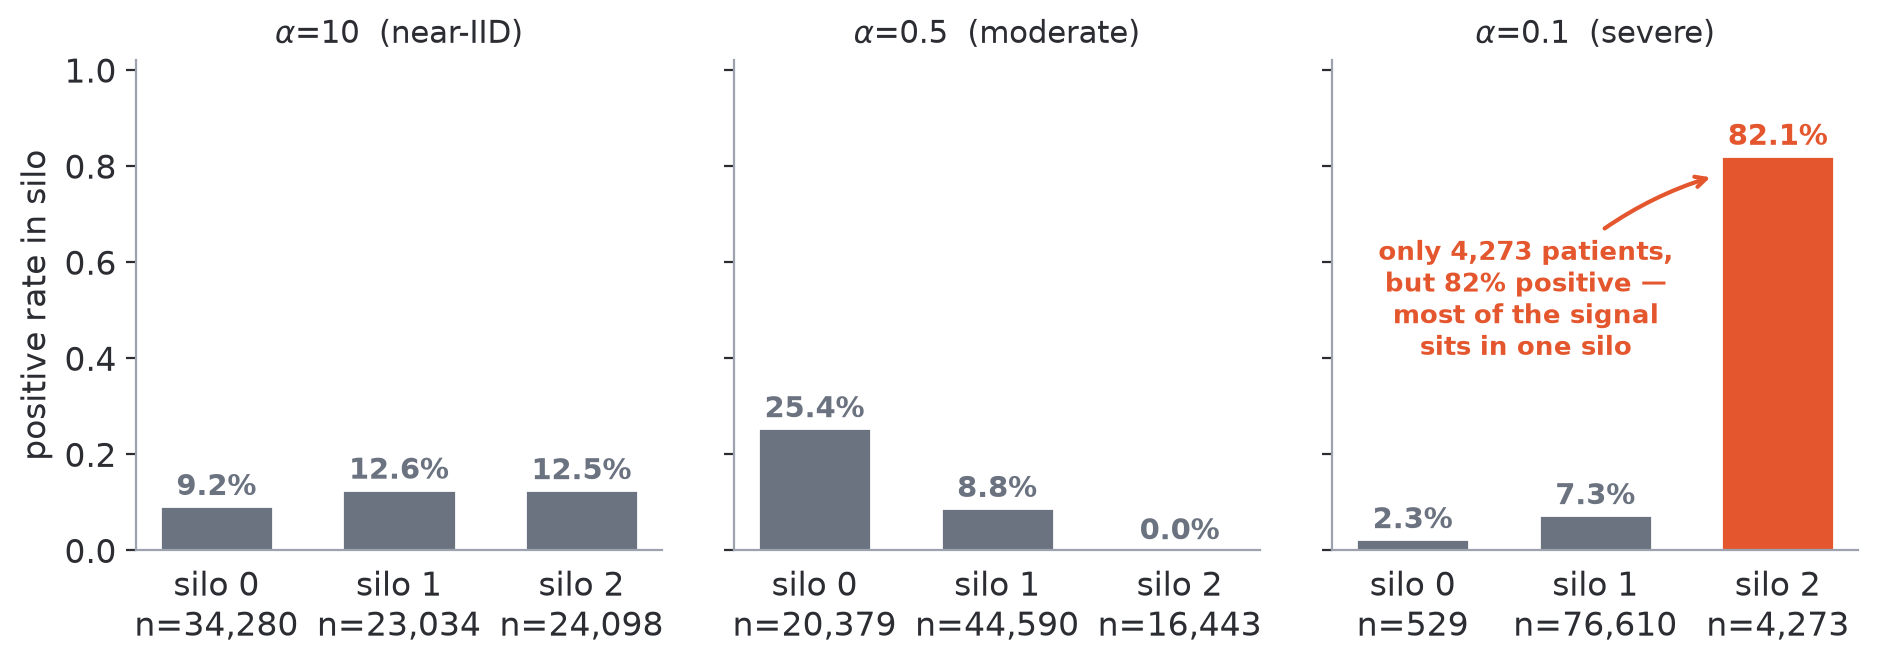
\includegraphics[width=\linewidth]{silo_composition.png}
\end{column}
\end{columns}
\end{frame}

% --------------------------------------------------------------------
\begin{frame}{Honest framing before any results}
\begin{alertblock}{Peak accuracy is explicitly \emph{not} the target}
The centralized ceiling on this task is $\approx$\,0.677 AUROC. That is
\textbf{not the object of study} and chasing it would optimize the wrong
quantity.
\end{alertblock}
\vspace{0.6em}
\begin{itemize}
\item What is under study is \textbf{how that accuracy moves}, and what
      governance costs, as patients exercise revocable consent.
\item The task's \textbf{low signal ceiling is convenient}: it guarantees
      measured degradation reflects \textbf{population change}, not
      under-fitting headroom.
\item The scientific weight rests entirely on the \textbf{deltas}.
\end{itemize}
\vspace{0.4em}
{\footnotesize I will return to this when discussing why nothing amplifies
under a stronger model --- it is the same fact, seen from the other side.}
\end{frame}

% ====================================================================
\section{Executed Results: The Utility Axis (RQ2)}
% ====================================================================

\begin{frame}{What is already executed}
\begin{center}\small
\begin{tabular}{p{5.6cm}p{4.4cm}l}
\toprule
\textbf{Study} & \textbf{Scale} & \textbf{Status}\\
\midrule
Centralized multi-model benchmark & 5 models, 5-fold CV & \done\\
Local-only floor (no federation)  & per-silo, $\alpha{=}0.5$ & \done\\
Five-method federated comparison  & 5 methods $\times$ 3 skew levels & \done\\
Three-regime consent-churn study  & 4 rates $\times$ 5 seeds & \done\\
Whole-silo exit + count-matched control & 2 skews $\times$ 5 seeds & \done\\
MLP amplification check (full grid rerun) & \textbf{200 training runs} & \done\\
\midrule
Systems-cost instrumentation (RQ1) & 3 backends & \planned\\
Joint frontier (RQ3), multi-project (RQ4) & --- & \planned\\
\bottomrule
\end{tabular}
\end{center}
\vspace{0.3em}
{\scriptsize Every figure in this section is regenerated directly from the
saved result files.}
\end{frame}

% --------------------------------------------------------------------
\begin{frame}{Anchor 1 --- the centralized ceiling and the local floor}
\begin{center}
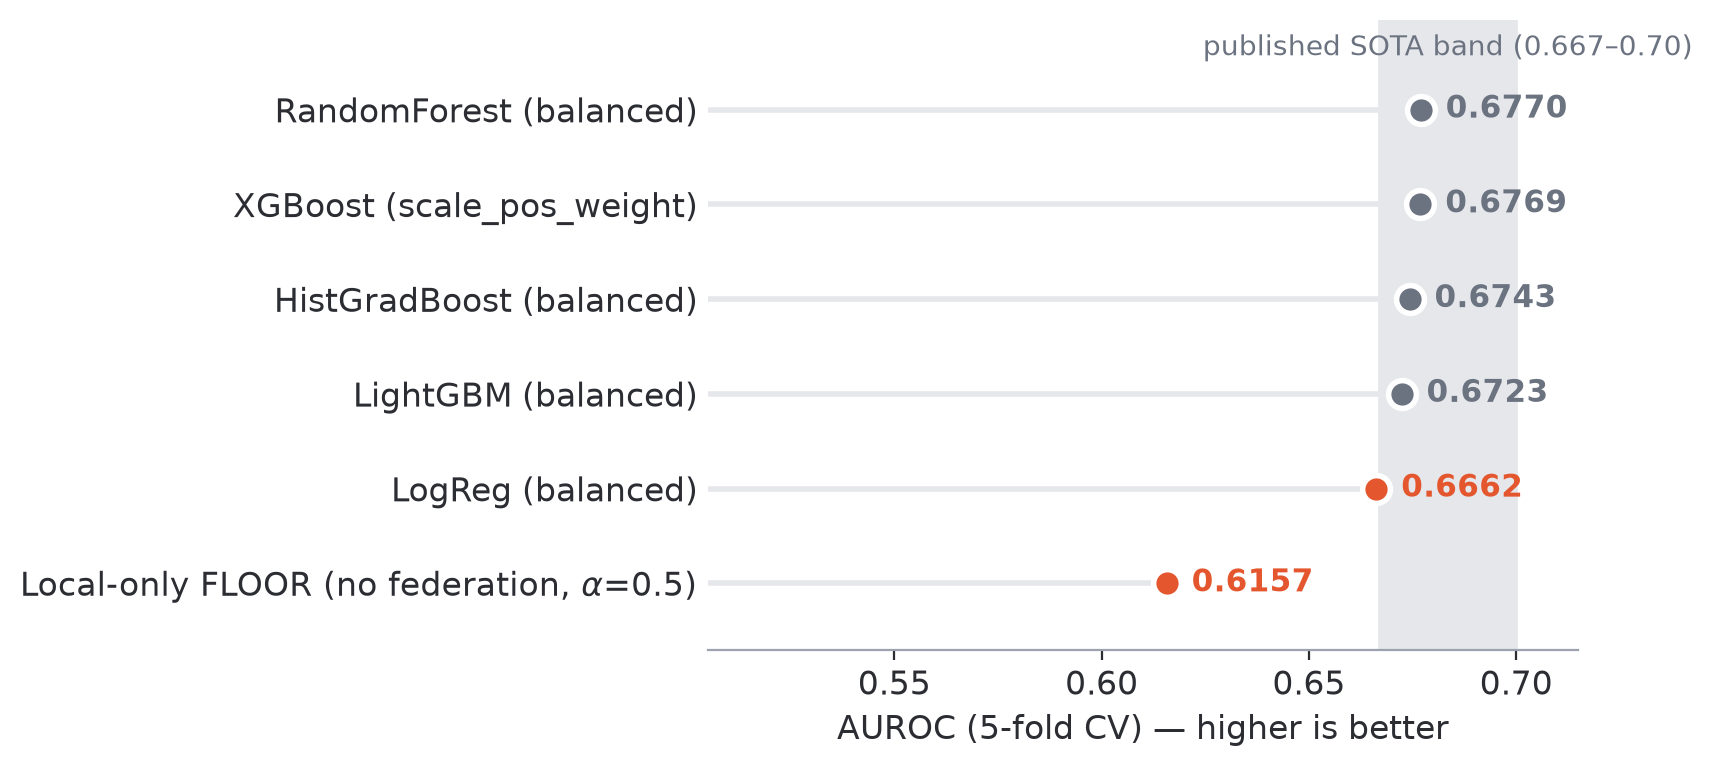
\includegraphics[width=0.76\linewidth]{ceiling.png}
\end{center}
\vspace{-0.4em}
\begin{itemize}\scriptsize
\item Best centralized: \textbf{0.6770} (Random Forest), inside the published
      \textbf{0.667--0.70} band for this task. Model choice barely moves
      AUROC --- the signal ceiling is genuinely low.
\item Local-only floor: \textbf{0.6157} mean (min \textbf{0.5159}). This is
      the cost of \emph{not} federating.
\end{itemize}
\end{frame}

% --------------------------------------------------------------------
\begin{frame}{Anchor 2 --- the federated ceiling is lower, and that is a result}
\begin{columns}[T]
\begin{column}{0.52\textwidth}
\begin{alertblock}{Trees are not weight-averageable}
Random Forest and XGBoost --- the two best centralized models --- \textbf{cannot
be averaged} across silos. FedAvg needs a parameter vector, not a forest.
\end{alertblock}
\vspace{0.5em}
So the \textbf{federated ceiling} is set by the best \emph{averageable} model:
\begin{itemize}\small
\item Logistic regression: \textbf{0.6662}
\item One-hidden-layer MLP: \textbf{0.6700}
\item Tree ceiling: \textbf{0.6770}
\end{itemize}
\end{column}
\begin{column}{0.46\textwidth}
\begin{exampleblock}{The first measured cost}
The \textbf{0.007--0.011 AUROC gap} between the tree ceiling and the
averageable ceiling is the first concrete, measured cost of federating this
task.\\[0.5em]
It is paid \textbf{before any patient withdraws consent at all}.
\end{exampleblock}
\vspace{0.3em}
{\footnotesize This is rarely stated in FL papers, which typically compare
federated-vs-centralized \emph{within} one model family and so never see it.}
\end{column}
\end{columns}
\end{frame}

% --------------------------------------------------------------------
\begin{frame}{Anchor 3 --- does the aggregation method matter?}
Five server-side aggregation strategies, same client, same data, same splits:
\vspace{0.4em}
\begin{center}\small
\begin{tabular}{lll}
\toprule
\textbf{Method} & \textbf{Mechanism} & \textbf{Reference}\\
\midrule
FedAvg    & weighted parameter average          & McMahan 2017\\
FedProx   & FedAvg $+$ client proximal term $\mu$ & Li 2020\\
FedAvgM   & server momentum on aggregated delta & Hsu 2019\\
FedAdam   & adaptive server optimizer (FedOpt)  & Reddi 2021\\
SCAFFOLD  & client control variates correct drift & Karimireddy 2020\\
\bottomrule
\end{tabular}
\end{center}
\vspace{0.6em}
\begin{block}{Implementation note that makes this fair}
All five operate on \textbf{one flat parameter vector}. Deltas, proximal
terms, and control variates are therefore \textbf{model-agnostic} --- swapping
the client model does not change the aggregation code at all. This matters
enormously later.
\end{block}
\end{frame}

% --------------------------------------------------------------------
\begin{frame}{Anchor 3 --- the answer: barely, until it is pathological}
\begin{center}
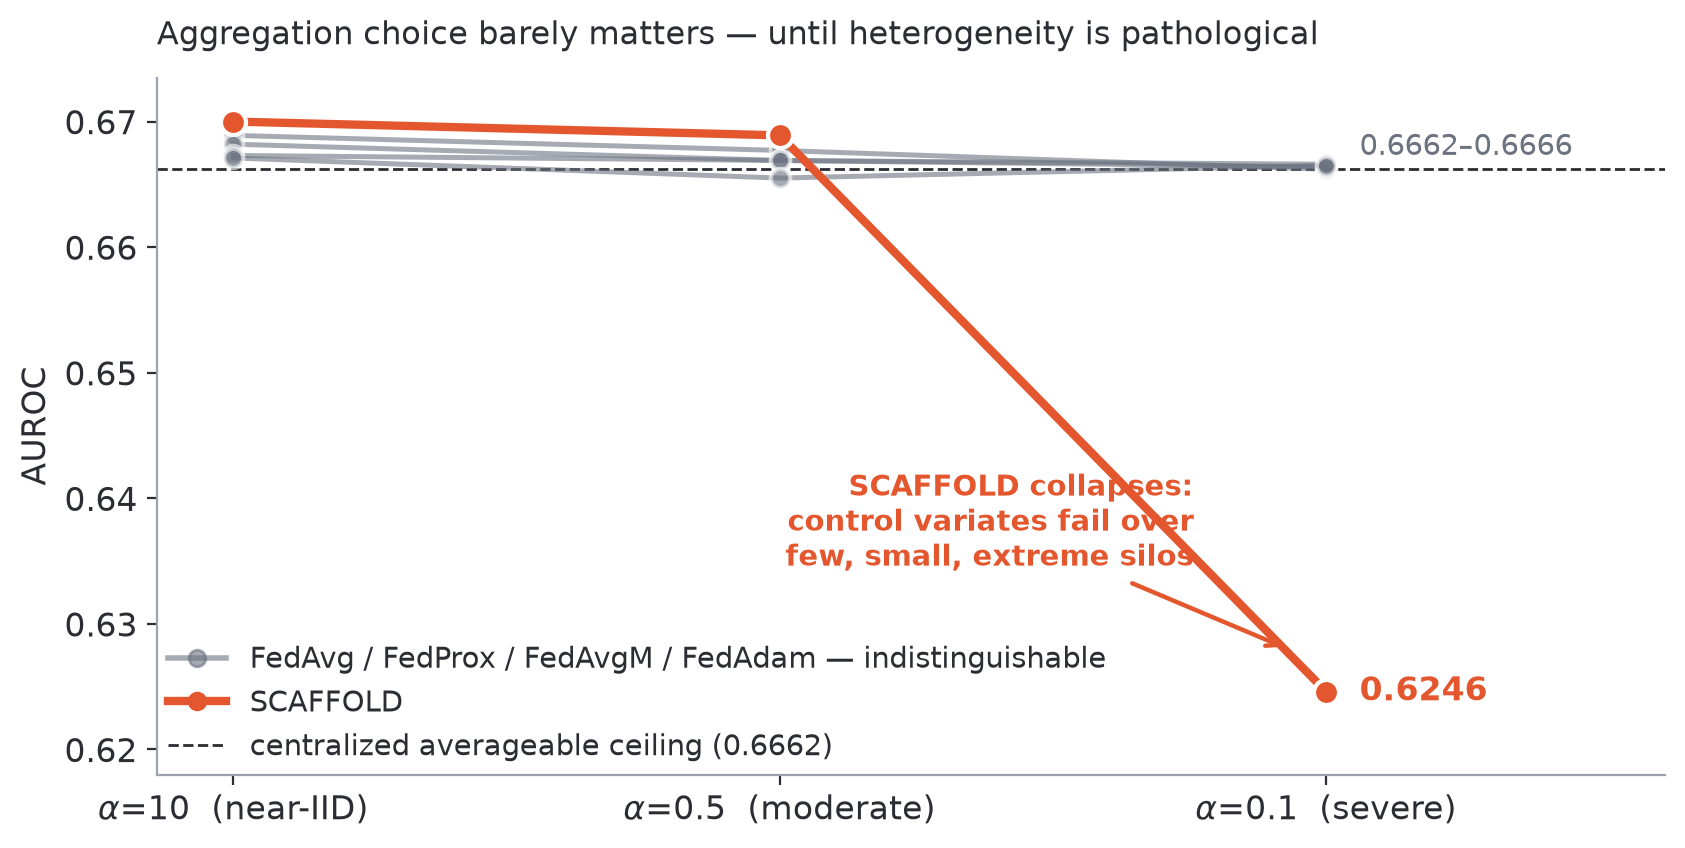
\includegraphics[width=0.74\linewidth]{fl_methods.png}
\end{center}
\vspace{-0.5em}
\begin{itemize}\scriptsize
\item Four methods are \textbf{statistically indistinguishable} at every skew
      level (0.6655--0.6700).
\item \hl{SCAFFOLD collapses at $\alpha{=}0.1$}: \textbf{0.6246}, a
      documented small-$K$ failure mode --- control variates are estimated
      from few, small, extreme silos and inject noise instead of correcting
      drift.
\end{itemize}
\end{frame}

% --------------------------------------------------------------------
\begin{frame}{Why FedAvg is the empirically justified instrument}
\begin{columns}[T]
\begin{column}{0.49\textwidth}
\begin{block}{The weak argument (not used)}
``FedAvg is the standard baseline.''\\[0.4em]
{\footnotesize True but lazy --- and a committee would rightly ask whether a
better aggregator would have absorbed the churn damage.}
\end{block}
\end{column}
\begin{column}{0.49\textwidth}
\begin{exampleblock}{The measured argument}
At $K{=}3$, \textbf{no alternative aggregator improves on FedAvg} --- and the
one that theoretically should (SCAFFOLD) \textbf{fails}.\\[0.4em]
So the churn results cannot be dismissed as ``you picked a weak aggregator.''
\end{exampleblock}
\end{column}
\end{columns}
\vspace{0.7em}
\begin{alertblock}{And its non-IID sensitivity is a \emph{feature} of the instrument}
FedAvg's known fragility under heterogeneity is precisely what makes consent
churn \textbf{visible} as a utility cost. A maximally robust aggregator would
be the wrong measuring device --- it would hide the very quantity being
measured.
\end{alertblock}
\end{frame}

% --------------------------------------------------------------------
\begin{frame}{The central experiment: three churn regimes}
The literature says ``churn.'' That word conflates \textbf{physically
distinct} phenomena. This thesis separates them.
\vspace{0.5em}
\begin{columns}[T]
\begin{column}{0.32\textwidth}
\begin{block}{1. Transient}
Patients withdraw, then \textbf{restore} consent later. Contributions
\textbf{re-enter} the population.\\[0.3em]
{\footnotesize \emph{Hypothesis: near-harmless.}}
\end{block}
\end{column}
\begin{column}{0.32\textwidth}
\begin{block}{2. Permanent}
Consent withdrawn \textbf{for good}, ramping to the target rate.\\[0.3em]
Split two ways: \textbf{random} (pure shrinkage) vs.\ \textbf{biased}
(positives leave first $\rightarrow$ distribution \emph{shifts}).
\end{block}
\end{column}
\begin{column}{0.32\textwidth}
\begin{block}{3. Whole-silo}
An \textbf{entire institution} exits --- a whole slice of the distribution
disappears at once.\\[0.3em]
{\footnotesize \emph{Hypothesis: dominates.}}
\end{block}
\end{column}
\end{columns}
\vspace{0.6em}
{\footnotesize Plus a fourth condition that is not a regime but a
\textbf{control} --- introduced in three slides, and it is the one that
carries the headline.}
\end{frame}

% --------------------------------------------------------------------
\begin{frame}[fragile]{How churn is injected (the mechanism)}
A \textbf{schedule} is a callable $r \mapsto [K$ active-index arrays$]$ giving,
for round $r$, the patients in each silo whose consent is currently active.
\vspace{0.3em}
\begin{exampleblock}{The seam}
\begin{semiverbatim}\scriptsize
federated_train(..., \alert{round_silos=schedule})

for r in range(rounds):
    cur = \alert{round_silos(r)}      # <- consent resolved per round
    sizes_r = [len(s) for s in cur]
    wts = sizes_r / sizes_r.sum()   # <- weights RECOMPUTED each round
    ...
\end{semiverbatim}
\end{exampleblock}
\vspace{0.3em}
\begin{itemize}\small
\item Silos with zero active patients contribute nothing that round.
\item Aggregation weights are \textbf{recomputed every round} from active
      sizes --- withdrawal changes the averaging, not just the data.
\item \hl{This same hook is where RQ1's gas/latency counters will attach.}
\end{itemize}
\end{frame}

% --------------------------------------------------------------------
\begin{frame}{Result 1 --- the rate sweep: per-patient churn is cheap}
\begin{center}
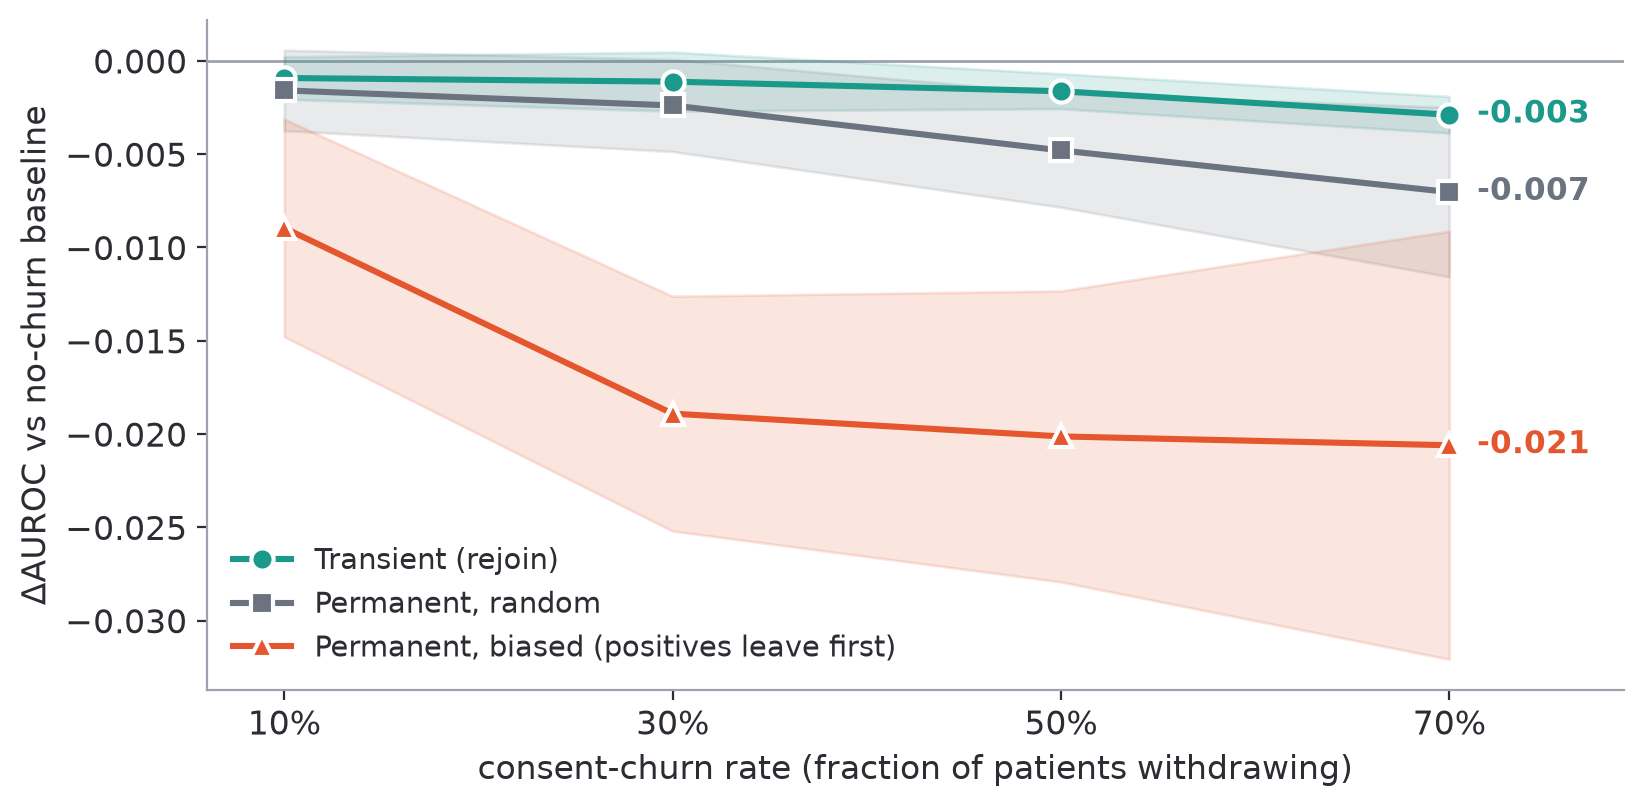
\includegraphics[width=0.70\linewidth]{churn_sweep.png}
\end{center}
\vspace{-0.5em}
\begin{itemize}\scriptsize
\item Transient churn at \textbf{70\%}: only \textbf{$-$0.003} AUROC.
      Contributions re-enter; the model barely notices.
\item Permanent \emph{random} at 70\%: \textbf{$-$0.007}. The population
      shrinks but does \textbf{not shift}.
\item Permanent \emph{biased} at 70\%: \textbf{$-$0.021} --- roughly
      \textbf{3$\times$} the random cost at identical headcount.
\end{itemize}
\end{frame}

% --------------------------------------------------------------------
\begin{frame}{Reading the rate sweep carefully}
\begin{columns}[T]
\begin{column}{0.49\textwidth}
\begin{exampleblock}{Finding A --- an honest null}
\textbf{Random per-patient churn is genuinely cheap} on this task. Even at
70\% withdrawal, the cost is under one AUROC point.\\[0.4em]
{\footnotesize This is a real, if undramatic, finding: consortia worrying
about attrition volume are worrying about the wrong thing.}
\end{exampleblock}
\end{column}
\begin{column}{0.49\textwidth}
\begin{alertblock}{Finding B --- where the cost lives}
The biased curve \textbf{separates immediately} and then
\textbf{plateaus} near $-$0.021 --- the damage is done early, once the
positive class is depleted, not accumulated linearly with headcount.\\[0.4em]
{\footnotesize The mechanism is \textbf{distribution shift}, not data volume.}
\end{alertblock}
\end{column}
\end{columns}
\vspace{0.6em}
{\footnotesize Note the widening error band on the biased regime --- with
positives preferentially removed, seed-to-seed variance grows as the effective
positive count shrinks. Stated, not hidden.}
\end{frame}

% --------------------------------------------------------------------
\begin{frame}{The isolation test: separating \emph{who} from \emph{how many}}
\begin{alertblock}{The confound}
A whole-silo exit removes a \textbf{distribution slice} \emph{and} a
\textbf{large headcount} at the same time. Any damage could be attributed to
either. The comparison is uninterpretable as stated.
\end{alertblock}
\vspace{0.6em}
\begin{exampleblock}{The control: \texttt{matched\_random}}
Remove \textbf{exactly the same number of patients} as the whole-silo exit ---
but draw them \textbf{uniformly at random across all silos}.\\[0.5em]
Headcount is now \textbf{held constant by construction}. Only \textbf{identity}
differs.
\end{exampleblock}
\vspace{0.5em}
{\footnotesize This is the single experiment the headline claim rests on. If
the two conditions came out equal, H2 would be dead.}
\end{frame}

% --------------------------------------------------------------------
\begin{frame}{Result 2 --- the headline}
\begin{center}
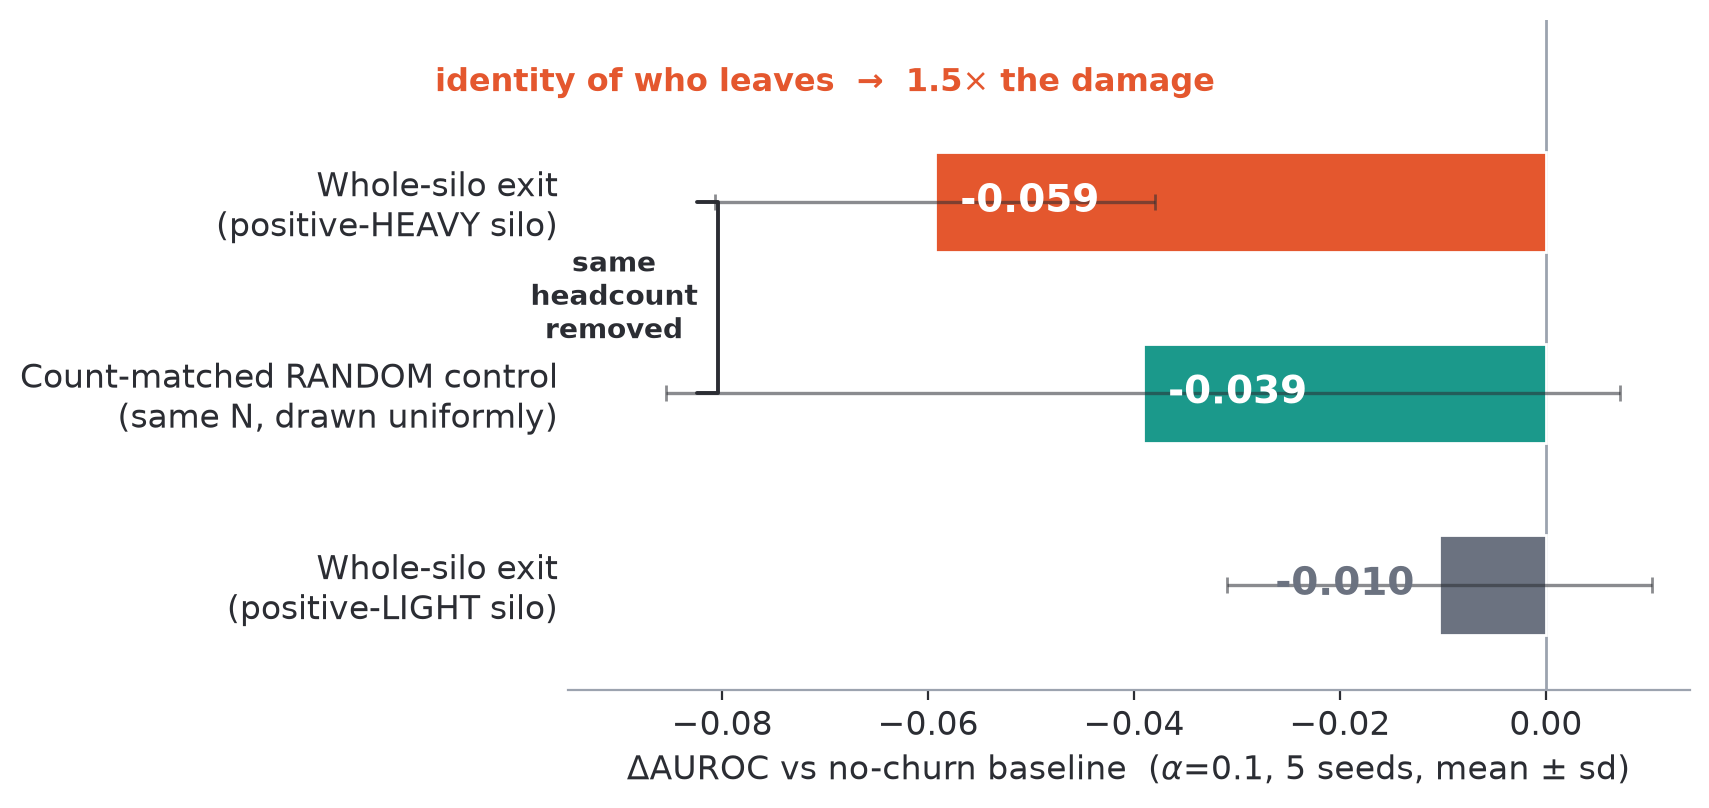
\includegraphics[width=0.86\linewidth]{isolation.png}
\end{center}
\vspace{-0.3em}
\begin{center}
\large
Same headcount removed. \hl{Identity carries the damage.}
\end{center}
\end{frame}

% --------------------------------------------------------------------
\begin{frame}{H2: confirmed}
\begin{center}
\Large
\emph{Who} leaves matters more than \emph{how many} leave.
\end{center}
\vspace{0.8em}
\begin{itemize}
\item Positive-heavy silo exit: \textbf{$-$0.059} AUROC.
\item Same headcount, drawn at random: \textbf{$-$0.039}.
\item Positive-\emph{light} silo exit: \textbf{$-$0.010} --- a
      \textbf{$\approx$6$\times$} spread between which institution leaves.
\end{itemize}
\vspace{0.6em}
\begin{alertblock}{Why this overturns the intuitive model}
The natural mental model --- and the one implicit in every consent-system
paper --- is a \textbf{headcount model}: more withdrawals, more damage. The
data says the damage is \textbf{distributional}. A consortium should not be
monitoring \emph{how many} patients have opted out; it should be monitoring
\emph{whether the opt-outs have changed the case mix}.
\end{alertblock}
\end{frame}

% --------------------------------------------------------------------
\begin{frame}{What I will not overclaim about this result}
\begin{columns}[T]
\begin{column}{0.49\textwidth}
\begin{alertblock}{The soft spot, stated plainly}
The seed-to-seed \textbf{standard deviations are large} relative to the gap:
\begin{itemize}\small
\item heavy exit: $-0.059$ \textbf{(sd 0.021)}
\item matched control: $-0.039$ \textbf{(sd 0.046)}
\end{itemize}
Five seeds on \emph{this specific comparison} is the weakest part of the
evidence.
\end{alertblock}
\end{column}
\begin{column}{0.49\textwidth}
\begin{exampleblock}{Why the claim still stands}
\begin{itemize}\small
\item The \textbf{direction} is consistent across \emph{both} client models
      (next section) --- an independent replication.
\item The \textbf{ordering} heavy $>$ matched $>$ light reproduces in every
      arm.
\item The \textbf{$\approx$6$\times$} light-vs-heavy spread is far outside
      noise.
\end{itemize}
\end{exampleblock}
\end{column}
\end{columns}
\vspace{0.5em}
\begin{block}{Committed remediation}
Finer seed counts and formal significance testing (McNemar; calibration via
expected calibration error) are folded into the funded work --- carried over
from our published benchmarking methodology.
\end{block}
\end{frame}

% ====================================================================
\section{Closing a Loophole: The Model-Capacity Check}
% ====================================================================

\begin{frame}{The obvious objection --- and I want to raise it myself}
\begin{alertblock}{The doubt}
Every churn number so far was measured on a \textbf{logistic-regression}
client.\\[0.5em]
Maybe the damage only \emph{looked} small because a \textbf{linear model is
too blunt to feel it}. A higher-capacity model might have far more to lose
under distribution shift --- in which case the ``cheap churn'' finding is an
artifact of a saturated model, not a property of consent churn.
\end{alertblock}
\vspace{0.6em}
\begin{itemize}
\item This objection, if correct, \textbf{invalidates the entire utility
      axis} --- and everything RQ3 would build on top of it.
\item So it was settled \textbf{before} anything else was built.
\end{itemize}
\end{frame}

% --------------------------------------------------------------------
\begin{frame}{The amplification check: design}
\begin{columns}[T]
\begin{column}{0.52\textwidth}
The \textbf{entire churn grid} was rerun with \textbf{two clients} on
\textbf{identical} partitions and schedules:
\begin{itemize}\small
\item the original \textbf{logistic regression};
\item a \textbf{one-hidden-layer MLP} (64 ReLU units, He init, lr 0.05).
\end{itemize}
\vspace{0.4em}
5 seeds $\times$ 3 regimes $\times$ 4 rates, plus both whole-silo exits and
the matched control, $\times$ 2 clients\\
$=$ \textbf{200 training runs}.
\end{column}
\begin{column}{0.46\textwidth}
\begin{exampleblock}{Two design choices that make it a fair test}
\textbf{1. The MLP is genuinely stronger}, not a handicapped stand-in: it
centralizes at \textbf{0.670}, \emph{above} the linear ceiling of 0.666 and
inside the published band.\\[0.5em]
\textbf{2. Aggregation is model-agnostic} --- both clients are one flat
parameter vector, so weighting, schedules, and harness are
\textbf{unchanged}. The two arms differ \emph{only} in the client model.
\end{exampleblock}
\end{column}
\end{columns}
\vspace{0.2em}
{\scriptsize Validity check: the logreg arm of the rerun \textbf{reproduces
the published churn table exactly}.}
\end{frame}

% --------------------------------------------------------------------
\begin{frame}{Result 3 --- no amplification}
\begin{center}
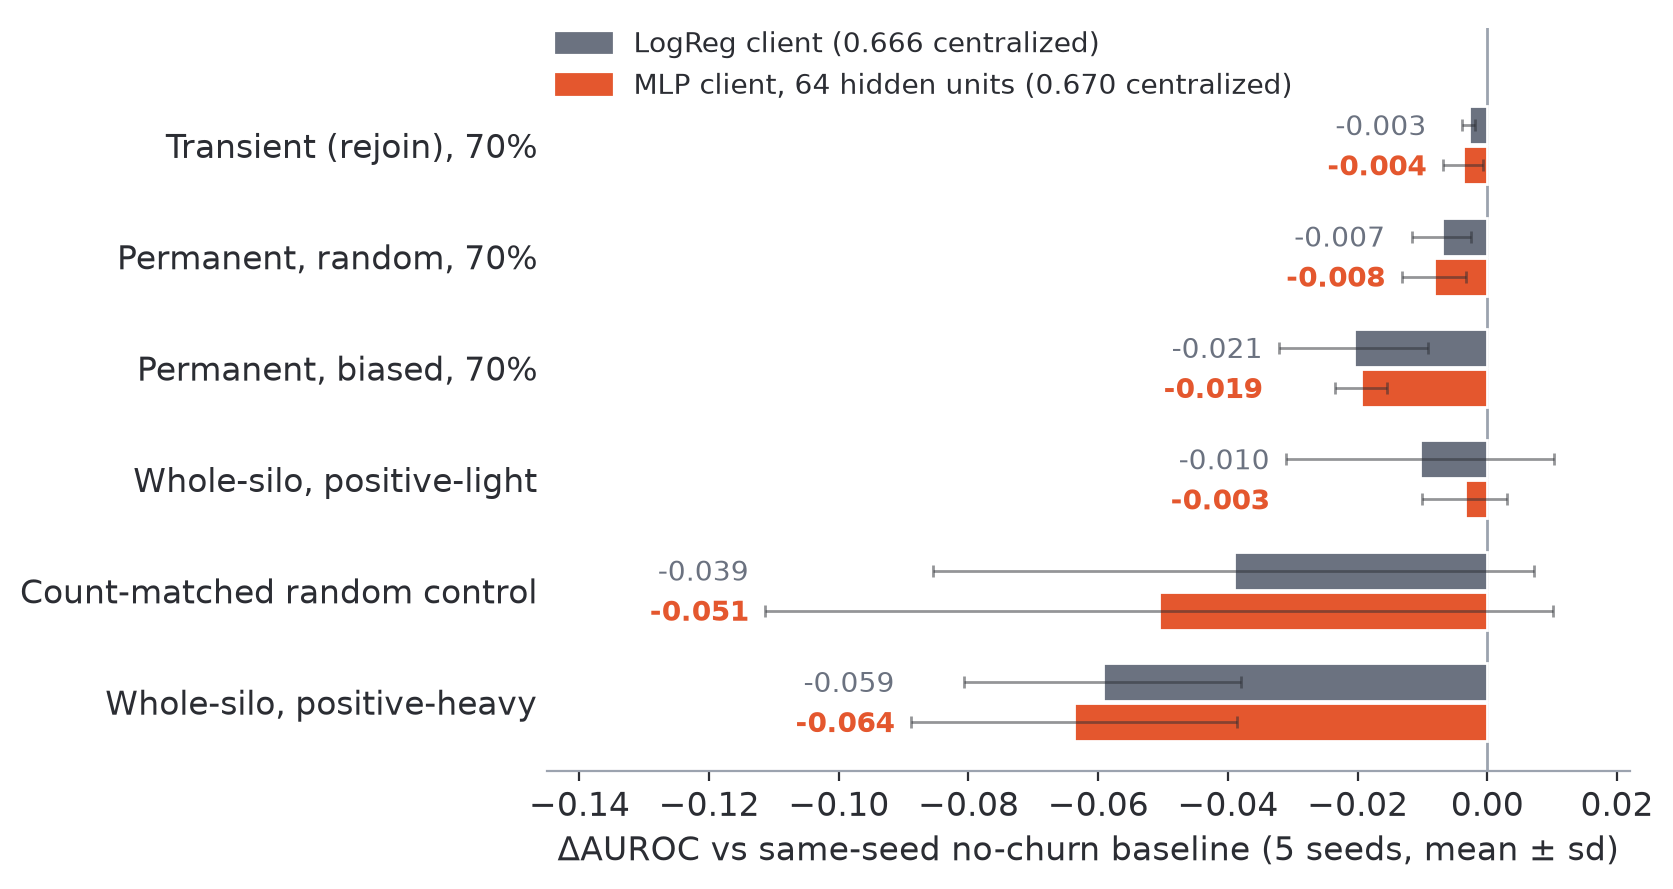
\includegraphics[width=0.68\linewidth]{mlp_deltas.png}
\end{center}
\vspace{-0.5em}
{\scriptsize Across all twelve rate-sweep cells the MLP deltas match the
logreg deltas \textbf{within one standard deviation} (amplification ratios
0.2--1.6). In the \textbf{biased} regime --- the one carrying the
mechanism --- the ratio is $\approx$\,\textbf{0.9}, i.e.\ marginally
\emph{smaller} on the MLP.}
\end{frame}

% --------------------------------------------------------------------
\begin{frame}{Three findings close the question}
\begin{enumerate}\setlength\itemsep{0.6em}
\item \textbf{No amplification --- the deltas are not a linear-model
      artifact.} The caveat resolved in the direction that
      \hl{strengthens} the result: the cost structure of consent churn is
      \textbf{model-independent} at this capacity.
\item \textbf{H2 survives the model swap.} On the MLP, the positive-heavy
      exit (\textbf{$-$0.064}) still dominates the count-matched control
      (\textbf{$-$0.051}) at identical headcount, and dwarfs the
      positive-light exit (\textbf{$-$0.003}) --- an $\approx$\,\textbf{18$\times$}
      who-leaves gap. ``Who leaves matters more'' is \textbf{not a property of
      logistic regression}.
\item \textbf{Why nothing amplifies: the \emph{task ceiling}, not the model
      class, bounds the deltas.} The MLP lifts the averageable ceiling only
      $0.666 \rightarrow 0.670$ against a tree ceiling of $0.677$. On a task
      \textbf{at its signal ceiling} there is little headroom for \emph{any}
      model to lose dramatically more under shift.
\end{enumerate}
\end{frame}

% --------------------------------------------------------------------
\begin{frame}{One secondary observation worth reporting}
\begin{block}{Higher capacity is slightly \emph{more} fragile at baseline}
The MLP's \textbf{no-churn} baseline is marginally worse under severe skew:
\begin{center}\small
$\alpha{=}0.1$: \quad MLP \textbf{0.629} \quad vs.\quad logreg \textbf{0.640}
\end{center}
Higher capacity overfits skewed silos marginally faster.
\end{block}
\vspace{0.7em}
\begin{itemize}
\item This cuts \emph{against} the ``use a bigger model'' reflex: at
      $K{=}3$ under severe heterogeneity, capacity is a mild liability
      \textbf{before churn is introduced at all}.
\item It also explains part of why the MLP's churn deltas do not amplify ---
      it starts from a lower, noisier baseline.
\end{itemize}
\end{frame}

% --------------------------------------------------------------------
\begin{frame}{The utility axis is closed}
\begin{exampleblock}{Summary of RQ2}
On a real clinical task at its signal ceiling:
\begin{itemize}
\item \textbf{per-patient consent churn stays cheap} ($-$0.003 to $-$0.007
      even at 70\% withdrawal);
\item \textbf{distribution-shifting churn is 3--6$\times$ more expensive};
\item and this holds \textbf{regardless of client capacity}.
\end{itemize}
\end{exampleblock}
\vspace{0.7em}
\begin{center}
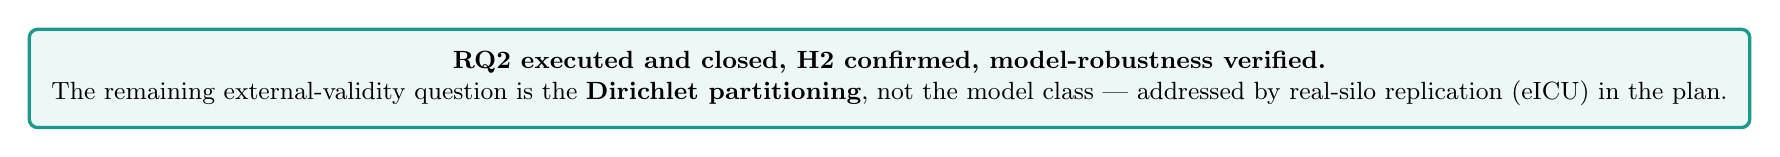
\begin{tikzpicture}[scale=1]
\node[draw=mTeal, very thick, rounded corners=3pt, fill=mTeal!8,
      inner sep=8pt, font=\small, align=center]
  {\textbf{RQ2 executed and closed, H2 confirmed, model-robustness verified.}\\
   The remaining external-validity question is the \textbf{Dirichlet
   partitioning}, not the model class --- addressed by real-silo replication
   (eICU) in the plan.};
\end{tikzpicture}
\end{center}
\end{frame}

% ====================================================================
\section{Proposed Work}
% ====================================================================

\begin{frame}{The critical path}
\begin{center}
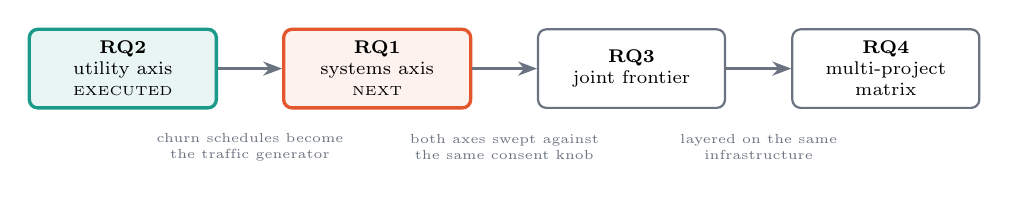
\begin{tikzpicture}[scale=0.95, transform shape,
  d/.style={draw=mTeal, very thick, rounded corners=3pt, fill=mTeal!10,
            minimum width=2.5cm, minimum height=1.05cm, font=\scriptsize,
            align=center},
  p/.style={draw=mGray, thick, rounded corners=3pt, fill=white,
            minimum width=2.5cm, minimum height=1.05cm, font=\scriptsize,
            align=center},
  n/.style={draw=mCoral, very thick, rounded corners=3pt, fill=mCoral!8,
            minimum width=2.5cm, minimum height=1.05cm, font=\scriptsize,
            align=center}]
  \node[d] (rq2) at (0,0)    {\textbf{RQ2}\\utility axis\\{\tiny EXECUTED}};
  \node[n] (rq1) at (3.4,0)  {\textbf{RQ1}\\systems axis\\{\tiny NEXT}};
  \node[p] (rq3) at (6.8,0)  {\textbf{RQ3}\\joint frontier};
  \node[p] (rq4) at (10.2,0) {\textbf{RQ4}\\multi-project\\matrix};
  \draw[-{Stealth[length=2.4mm]}, mGray, thick] (rq2) -- (rq1);
  \draw[-{Stealth[length=2.4mm]}, mGray, thick] (rq1) -- (rq3);
  \draw[-{Stealth[length=2.4mm]}, mGray, thick] (rq3) -- (rq4);
  \node[font=\tiny, text=mGray, align=center] at (1.7,-1.05)
     {churn schedules become\\the traffic generator};
  \node[font=\tiny, text=mGray, align=center] at (5.1,-1.05)
     {both axes swept against\\the same consent knob};
  \node[font=\tiny, text=mGray, align=center] at (8.5,-1.05)
     {layered on the same\\infrastructure};
\end{tikzpicture}
\end{center}
\vspace{0.5em}
\begin{alertblock}{The key economy}
RQ1 does \textbf{not} need new experimental design. The
\textbf{already-built churn schedules} generate the on-chain transaction
traffic. The same knob that drives the utility axis drives the systems axis
--- which is what makes a \emph{joint} frontier possible at all.
\end{alertblock}
\end{frame}

% --------------------------------------------------------------------
\begin{frame}{RQ1 --- what gets instrumented}
Every federated round is instrumented to decompose its cost into
\textbf{compute} and \textbf{governance}.
\vspace{0.5em}
\begin{columns}[T]
\begin{column}{0.48\textwidth}
\begin{block}{Governance covers}
\begin{itemize}\small
\item \textbf{Consent-set resolution} --- querying the ledger for who is
      active this round
\item \textbf{Grant/revoke transactions} --- gas per operation
\item \textbf{Encrypted-record retrieval} --- IPFS fetch latency
\end{itemize}
\end{block}
\end{column}
\begin{column}{0.48\textwidth}
\begin{block}{Measured per round}
\begin{itemize}\small
\item wall-clock latency (distribution, not mean)
\item gas / monetary cost
\item bandwidth
\item failure rate under congestion
\end{itemize}
\end{block}
\end{column}
\end{columns}
\vspace{0.4em}
\begin{exampleblock}{Attachment point}
\small The \texttt{round\_silos} hook shown earlier --- the same seam the
churn schedules already use. \textbf{No architectural change is required.}
\end{exampleblock}
\end{frame}

% --------------------------------------------------------------------
\begin{frame}{RQ1 --- the sweep}
\begin{center}\small
\begin{tabular}{p{3.3cm}p{8.4cm}}
\toprule
\textbf{Swept parameter} & \textbf{Range and rationale}\\
\midrule
Consent-churn rate &
  10--70\%, reusing the executed schedules --- ties the systems axis to the
  utility axis on \emph{one shared knob}\\
\addlinespace
Consent-refresh cadence &
  every round $\rightarrow$ every $n$ rounds --- the amortization dimension
  that H1 predicts will become necessary\\
\addlinespace
Federation size $K$ &
  small $\rightarrow$ hospital-scale, driven by \textbf{Synthea} populations\\
\addlinespace
Chain backend &
  \textbf{local} (Ganache), \textbf{permissioned}, \textbf{public} (Sepolia)
  --- spanning the 0.05\,s to 108\,s range already measured\\
\bottomrule
\end{tabular}
\end{center}
\vspace{0.5em}
\begin{alertblock}{Reporting commitment}
\textbf{Distributions, not means.} Public-chain latency is heavy-tailed and we
have already observed outright transaction failures under congestion --- a
mean would erase exactly the behavior that determines feasibility.
\end{alertblock}
\end{frame}

% --------------------------------------------------------------------
\begin{frame}{RQ1 --- what a positive result looks like}
\begin{exampleblock}{The H1 objective}
Locate the \textbf{infeasibility threshold}: the churn rate beyond which
per-round on-chain consent enforcement \textbf{cannot keep up}, and consent
must be \textbf{amortized across rounds}.
\end{exampleblock}
\vspace{0.6em}
\begin{itemize}
\item The threshold is expected to be \textbf{backend-dependent} --- and the
      published measurements already suggest the spread is enormous
      (0.05\,s local vs.\ up to 108\,s public per operation).
\item Amortization is not free: it introduces \textbf{consent staleness}.
      Training proceeds on a consent set that is knowingly out of date.
\item \hl{The deliverable is the amortization--staleness tradeoff curve} ---
      how much staleness must be accepted to stay feasible, per backend.
\end{itemize}
\vspace{0.2em}
{\scriptsize An ethically loaded quantity --- and exactly what the
architectural literature never surfaces.}
\end{frame}

% --------------------------------------------------------------------
\begin{frame}{RQ3 --- assembling the joint frontier}
\begin{columns}[T]
\begin{column}{0.5\textwidth}
Both axes are swept against the \textbf{same} consent knobs, then plotted
against each other.
\vspace{0.4em}
\begin{itemize}\small
\item $x$: governance cost per round (from RQ1)
\item $y$: model utility (from RQ2)
\item parameterized by: churn rate, \textbf{refresh cadence}, $K$, backend
\end{itemize}
\vspace{0.4em}
\begin{alertblock}{H3 --- the knee}
Some refresh cadences should recover \textbf{most} of the utility of
per-round enforcement at \textbf{a fraction} of the cost.
\end{alertblock}
\end{column}
\begin{column}{0.48\textwidth}
\begin{exampleblock}{Why RQ2's result sharpens this}
The utility axis already told us \textbf{where utility is sensitive}: to
\textbf{distribution shift}, not headcount.\\[0.5em]
So the frontier's shape should be governed by how quickly consent staleness
lets the \textbf{case mix} drift --- not by how many revocations accumulate.\\[0.5em]
That is a \textbf{sharper, falsifiable prediction} than we could have made
before RQ2 was executed.
\end{exampleblock}
\end{column}
\end{columns}
\end{frame}

% --------------------------------------------------------------------
\begin{frame}{RQ4 --- multi-project consent}
\begin{columns}[T]
\begin{column}{0.5\textwidth}
A patient is rarely in \emph{one} study. The consent layer must govern a
\textbf{patient\,$\times$\,study matrix}.
\vspace{0.4em}
\begin{itemize}\small
\item Implemented at the \textbf{contract/ledger level}.
\item Measure the \textbf{marginal governance cost} per additional study.
\end{itemize}
\vspace{0.4em}
\begin{alertblock}{H4}
Overhead is \textbf{bounded and sub-linear}, because consent state is
\textbf{shared infrastructure}, not per-study duplication.
\end{alertblock}
\end{column}
\begin{column}{0.48\textwidth}
\begin{center}
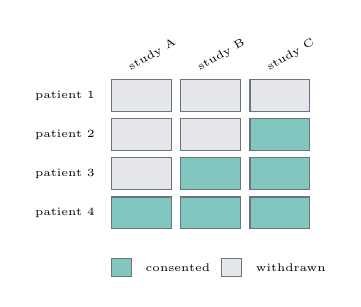
\begin{tikzpicture}[scale=0.80, transform shape]
  \foreach \i in {0,1,2,3}{
    \foreach \j in {0,1,2}{
      \pgfmathparse{(\i+\j)*7 > 20 ? 1 : 0}
      \ifnum\pgfmathresult=1
        \fill[mTeal!55] (\j*1.1,-\i*0.62) rectangle ++(0.95,0.5);
      \else
        \fill[mLight] (\j*1.1,-\i*0.62) rectangle ++(0.95,0.5);
      \fi
      \draw[mGray, thin] (\j*1.1,-\i*0.62) rectangle ++(0.95,0.5);}}
  \foreach \j/\l in {0/study A, 1/study B, 2/study C}{
    \node[font=\tiny, rotate=30, anchor=west] at (\j*1.1+0.18,0.62) {\l};}
  \foreach \i/\l in {0/patient 1, 1/patient 2, 2/patient 3, 3/patient 4}{
    \node[font=\tiny, anchor=east] at (-0.14,-\i*0.62+0.25) {\l};}
  % legend, below the grid so it cannot run off the column
  \fill[mTeal!55] (0,-2.62) rectangle ++(0.32,0.28);
  \draw[mGray, thin] (0,-2.62) rectangle ++(0.32,0.28);
  \node[font=\tiny, anchor=west] at (0.42,-2.48) {consented};
  \fill[mLight] (1.75,-2.62) rectangle ++(0.32,0.28);
  \draw[mGray, thin] (1.75,-2.62) rectangle ++(0.32,0.28);
  \node[font=\tiny, anchor=west] at (2.17,-2.48) {withdrawn};
\end{tikzpicture}
\end{center}
\vspace{0.2em}
{\footnotesize Demonstrates generality \textbf{without building a second
end-to-end system} --- the marginal cost is the evidence.}
\end{column}
\end{columns}
\end{frame}

% ====================================================================
\section{Timeline, Risks, and Limitations}
% ====================================================================

\begin{frame}{Timeline}
\begin{center}\scriptsize
\begin{tabular}{p{2.5cm}p{9.6cm}}
\toprule
\textbf{Period} & \textbf{Milestone}\\
\midrule
2024 \textcolor{mTeal}{\emph{(done)}} &
  Component papers published: Spark benchmarking, blockchain/IPFS consent
  layer, supply-chain regime shift.\\
\addlinespace
Spring 2026 \textcolor{mTeal}{\emph{(done)}} &
  Thesis framing finalized (two-axis cost of autonomy); primary dataset locked
  (Diabetes 130); Synthea confined to the systems axis.\\
\addlinespace
Summer 2026 \textcolor{mTeal}{\emph{(done)}} &
  Utility axis executed: centralized ceiling, five-method federated
  comparison, three-regime churn study with the count-matched isolation test
  (H2 confirmed), and the MLP amplification check.\\
\midrule
Fall 2026 &
  \textbf{Systems-cost axis (RQ1)}: gas/latency/bandwidth instrumentation on
  the per-round hook across local, permissioned, and public backends; Synthea
  scaling to locate the H1 threshold.\\
\addlinespace
Winter 2026--\newline Spring 2027 &
  \textbf{Joint frontier (RQ3)}: both axes swept against the shared churn
  knob; locate the amortization knee. \textbf{Multi-project matrix (RQ4)}.\\
\addlinespace
Spring--\newline Summer 2027 &
  Robustness replication on real hospital silos (eICU); dissertation writing
  and defense.\\
\bottomrule
\end{tabular}
\end{center}
\end{frame}

% --------------------------------------------------------------------
\begin{frame}{Risks and mitigations}
\begin{center}\scriptsize
\begin{tabular}{p{4.3cm}p{7.9cm}}
\toprule
\textbf{Risk} & \textbf{Mitigation}\\
\midrule
Public-testnet volatility makes RQ1 measurements irreproducible &
  Report distributions across time-of-day (methodology already validated);
  anchor with the deterministic local backend; treat congestion failures as
  \emph{data}, not noise\\
\addlinespace
Dirichlet partitions are not real hospital boundaries &
  Real-silo replication on \textbf{eICU} is scheduled, not optional; the
  partitioning is named as the remaining external-validity threat\\
\addlinespace
Utility deltas are moderate in absolute terms &
  Already de-risked: the model-class explanation was tested and
  \textbf{eliminated}; the deltas are bounded by the \emph{task ceiling},
  which is a property of the domain\\
\addlinespace
Synthea populations do not reflect real consent behavior &
  Synthea is confined to the systems axis, where only \textbf{volume and
  payload size} matter and signal realism is irrelevant\\
\addlinespace
Frontier turns out to be linear (H3 false) &
  A linear frontier is still a publishable measurement --- it would mean
  amortization buys nothing, which contradicts current deployment practice\\
\bottomrule
\end{tabular}
\end{center}
\end{frame}

% --------------------------------------------------------------------
\begin{frame}{Limitations, stated plainly}
\begin{itemize}\setlength\itemsep{0.5em}
\item The federation is \textbf{simulated}, not a live multi-hospital
      deployment.
\item Silos are \textbf{Dirichlet partitions of one cohort}, not real
      hospital boundaries. This is now the \textbf{primary} external-validity
      question --- the model-class alternative having been ruled out.
\item Measured utility magnitudes are \textbf{moderated} by the large cohort
      and by AUROC's rank-robustness.
\item Synthetic data is confined to the systems axis --- by design, but it
      does mean the systems axis is not driven by real consent behavior.
\item The Year-1 system claims \textbf{consent governance and data autonomy},
      \textbf{not formal privacy}.
\end{itemize}
\vspace{0.4em}
{\footnotesize Each of these is either scheduled for remediation (eICU,
DP thrust) or is an accepted, named boundary of the contribution.}
\end{frame}

% --------------------------------------------------------------------
\begin{frame}{Future work beyond the proposal}
\begin{enumerate}\setlength\itemsep{0.45em}
\item \textbf{Privacy that earns the word.} Compose DP-SGD and/or secure
      aggregation, adding a \textbf{third axis} (noise $\rightarrow$ accuracy
      loss) to the same frontier.
\item \textbf{Federated unlearning.} The \emph{biased permanent withdrawal}
      regime is the natural setting: when a patient revokes, can their
      contribution be \textbf{removed} from an already-trained model rather
      than merely excluded going forward?
\item \textbf{Real hospital silos.} eICU replication, replacing Dirichlet
      partitions with genuine institutional boundaries.
\item \textbf{Image scale.} Cervical images (SipakMed), where the published
      Spark/CNN pipeline is \textbf{justified} by the compute-placement rule.
\end{enumerate}
\end{frame}

% --------------------------------------------------------------------
\begin{frame}{Summary}
\begin{columns}[T]
\begin{column}{0.49\textwidth}
\begin{exampleblock}{What is done \donelight}
\begin{itemize}\small
\item Centralized ceiling, local floor, federated ceiling --- all measured
\item Five aggregation methods compared; FedAvg empirically justified
\item Three churn regimes separated and swept
\item \textbf{H2 confirmed} by count-matched isolation test
\item \textbf{Model-independence verified} (200 runs)
\end{itemize}
\end{exampleblock}
\end{column}
\begin{column}{0.49\textwidth}
\begin{block}{What is proposed \planned}
\begin{itemize}\small
\item RQ1: on-chain governance instrumentation across three backends
\item H1 infeasibility threshold and the amortization--staleness tradeoff
\item RQ3: the joint cost--utility frontier and its knee
\item RQ4: multi-project consent matrix, marginal cost per study
\end{itemize}
\end{block}
\end{column}
\end{columns}
\vspace{0.6em}
\begin{center}
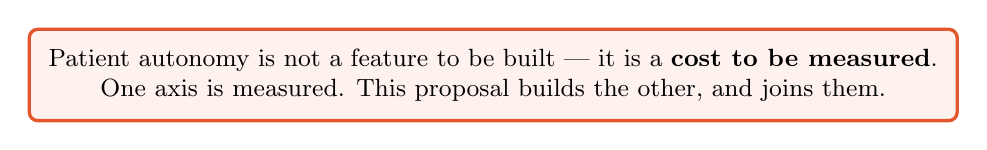
\begin{tikzpicture}
\node[draw=mCoral, very thick, rounded corners=3pt, fill=mCoral!8,
      inner sep=7pt, font=\small, align=center]
  {Patient autonomy is not a feature to be built --- it is a
   \textbf{cost to be measured}.\\
   One axis is measured. This proposal builds the other, and joins them.};
\end{tikzpicture}
\end{center}
\end{frame}

% --------------------------------------------------------------------
\begin{frame}[standout]
Thank you.\\[0.6em]
{\large Questions?}
\end{frame}

% ====================================================================
\appendix
\section{Backup Slides}
% ====================================================================

\begin{frame}{Backup --- full churn results table}
\begin{center}\small
\begin{tabular}{lrr}
\toprule
Condition & LogReg client & MLP client\\
\midrule
Transient (rejoin), 70\% churn                   & $-0.003$ (0.001) & $-0.004$ (0.003)\\
Permanent, random, 70\%                          & $-0.007$ (0.005) & $-0.008$ (0.005)\\
Permanent, biased, 70\%                          & $-0.021$ (0.011) & $-0.020$ (0.004)\\
Whole-silo exit, positive-light ($\alpha{=}0.1$) & $-0.010$ (0.021) & $-0.004$ (0.007)\\
Whole-silo exit, positive-heavy ($\alpha{=}0.1$) & $-0.059$ (0.021) & $-0.064$ (0.025)\\
\emph{Count-matched random control} ($\alpha{=}0.1$) & $-0.039$ (0.046) & $-0.051$ (0.061)\\
\midrule
\multicolumn{3}{l}{\emph{No-churn baselines}}\\
$\alpha{=}0.5$                                   & $0.6587$ & $0.6575$\\
$\alpha{=}0.1$                                   & $0.6404$ & $0.6290$\\
\bottomrule
\end{tabular}
\end{center}
\vspace{0.4em}
{\footnotesize $\Delta$AUROC vs.\ the \textbf{same-seed} no-churn baseline
under identical partitions and consent schedules; mean (sd) over five seeds.}
\end{frame}

% --------------------------------------------------------------------
\begin{frame}{Backup --- hyperparameters}
\begin{columns}[T]
\begin{column}{0.48\textwidth}
\begin{block}{Federated setup}
\begin{itemize}\small
\item Rounds: \textbf{40}; local epochs: \textbf{1}
\item Batch size: \textbf{256}; $L_2$: \textbf{1e-4}
\item Class weighting: \textbf{on} (global, from train split)
\item $K = 3$ silos; seeds \textbf{0--4}
\item Learning rate: \textbf{0.1} (logreg), \textbf{0.05} (MLP)
\end{itemize}
\end{block}
\end{column}
\begin{column}{0.48\textwidth}
\begin{block}{Method-specific}
\begin{itemize}\small
\item FedProx: $\mu = 0.1$
\item FedAvgM: server momentum $0.9$
\item FedAdam: server lr $0.05$, $\beta_1{=}0.9$, $\beta_2{=}0.99$,
      $\epsilon{=}$1e-3
\item SCAFFOLD: Option II control-variate update
\item Biased schedule: withdrawal bias $= 8.0\times$ for positives
\end{itemize}
\end{block}
\end{column}
\end{columns}
\vspace{0.4em}
{\footnotesize MLP: 1 hidden layer, 64 ReLU units, He initialization,
flat parameter vector of size $n_f \cdot H + 2H + 1$.}
\end{frame}

% --------------------------------------------------------------------
\begin{frame}{Backup --- the four churn schedules}
\begin{center}\small
\begin{tabular}{p{2.7cm}p{9.4cm}}
\toprule
\textbf{Schedule} & \textbf{Mechanism}\\
\midrule
\texttt{transient} &
  Each round independently deactivates $\approx$\,rate of every silo;
  patients \textbf{can return}. Fresh RNG per round.\\
\addlinespace
\texttt{permanent} &
  Cumulative, irreversible withdrawal ramping to rate by the final round.
  Withdrawal order \textbf{random within each silo} $\Rightarrow$ shrinkage
  without shift.\\
\addlinespace
\texttt{biased\_permanent} &
  Same ramp, but positive-class patients withdraw preferentially
  ($8\times$), via a Gumbel-top-$k$ / exponential-race weighted ordering
  $\Rightarrow$ \textbf{shifts the class distribution}.\\
\addlinespace
\texttt{whole\_silo} &
  Named silos hold \textbf{no} active patients from \texttt{depart\_round} on.\\
\addlinespace
\texttt{matched\_random} &
  Removes \textbf{exactly} \texttt{n\_remove} patients drawn uniformly across
  \emph{all} silos --- the count-matched control.\\
\bottomrule
\end{tabular}
\end{center}
\end{frame}

% --------------------------------------------------------------------
\begin{frame}{Backup --- why SCAFFOLD collapses at $\alpha{=}0.1$}
\begin{itemize}
\item SCAFFOLD corrects client drift using \textbf{control variates}
      $c_i$ estimated from each client's local updates.
\item Those estimates are only reliable when clients have
      \textbf{enough data} and \textbf{enough participation} to average out
      noise.
\item At $\alpha{=}0.1$, $K{=}3$: one silo has \textbf{529 patients at 2.3\%
      positive}, another \textbf{4,273 at 82\% positive}.
\item Control variates estimated from such extreme, small silos
      \textbf{inject noise} rather than correcting drift --- a documented
      small-$K$ failure mode.
\end{itemize}
\vspace{0.5em}
\begin{block}{Why this is reported rather than dropped}
It is a \textbf{diagnostic}, not a nuisance: it confirms the
$\alpha{=}0.1$ regime is genuinely pathological, which is what makes it the
right stress condition for the whole-silo exit test.
\end{block}
\end{frame}

% --------------------------------------------------------------------
\begin{frame}{Backup --- full five-method federated results}
\begin{center}\small
\begin{tabular}{lrrrr}
\toprule
& \multicolumn{4}{c}{\textbf{AUROC}}\\
\cmidrule(l){2-5}
Method & $\alpha{=}10$ & $\alpha{=}0.5$ & $\alpha{=}0.1$ & PR-AUC ($\alpha{=}0.1$)\\
\midrule
FedAvg   & 0.6689 & 0.6677 & 0.6662 & 0.2110\\
FedProx  & 0.6682 & 0.6669 & 0.6664 & 0.2106\\
FedAvgM  & 0.6673 & 0.6669 & 0.6666 & 0.2099\\
FedAdam  & 0.6671 & 0.6655 & 0.6665 & 0.2112\\
SCAFFOLD & 0.6700 & 0.6689 & \textbf{0.6246} & \textbf{0.1758}\\
\midrule
\multicolumn{5}{l}{\emph{Reference anchors}}\\
Centralized averageable ceiling (logreg) & \multicolumn{4}{l}{0.6662}\\
Best centralized overall (Random Forest) & \multicolumn{4}{l}{0.6770}\\
Local-only floor ($\alpha{=}0.5$, mean)  & \multicolumn{4}{l}{0.6157 (min 0.5159)}\\
\bottomrule
\end{tabular}
\end{center}
\end{frame}

% --------------------------------------------------------------------
\begin{frame}{Backup --- Dirichlet partition composition}
\begin{center}
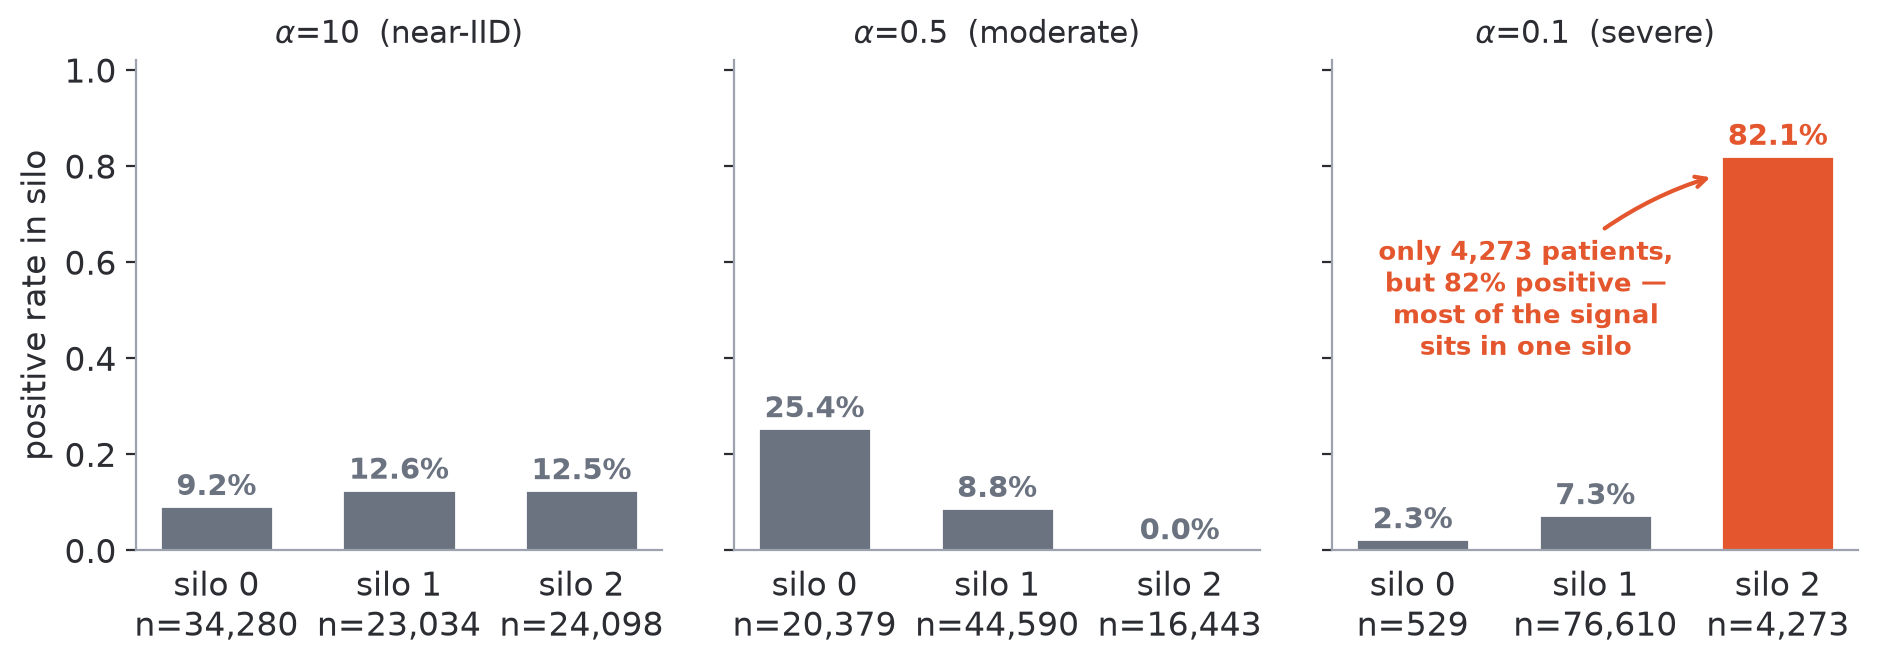
\includegraphics[width=0.9\linewidth]{silo_composition.png}
\end{center}
\vspace{-0.2em}
{\footnotesize At $\alpha{=}0.5$, silo 2 receives \textbf{zero} positive
cases --- an extreme but legitimate draw that the class-weighted trainer must
handle (its contribution to the positive gradient is nil, and aggregation
weights are recomputed from active sizes each round).}
\end{frame}

% --------------------------------------------------------------------
\begin{frame}{Backup --- blockchain cost detail}
\begin{center}\small
\begin{tabular}{lrr}
\toprule
\textbf{Ganache (local, single node)} & Time (s) & Cost (ETH)\\
\midrule
Add permission     & 0.052096 & 0.00099022\\
Revoke permission  & 0.070517 & 0.00119175\\
\midrule
\textbf{Sepolia (public testnet)} & \multicolumn{2}{l}{}\\
\midrule
Add, fastest        & 8.84 & ---\\
Revoke, fastest     & 12.01 & ---\\
Add, peak (12\,PM)  & 55.09 & up to 0.0029\\
Revoke, peak (1--2\,AM) & 107.99 & up to 0.019805\\
\bottomrule
\end{tabular}
\end{center}
\vspace{0.5em}
{\footnotesize Congestion between 6--9\,AM CT produced outright transaction
\textbf{failures} under the configured wallet settings. IPFS retrieval
typically under 0.3\,s. Revoke is consistently costlier than add on both
backends --- a detail that matters, since \textbf{revocation is the operation
patient autonomy generates}.}
\end{frame}

% --------------------------------------------------------------------
\begin{frame}{Backup --- reproducibility}
\begin{itemize}
\item All experiments run from a single conda environment
      (\texttt{thesis}, Python 3.11).
\item \texttt{01\_baseline\_fullscale/} --- preprocessing, multi-model
      centralized benchmark, five FL aggregation methods.
\item \texttt{02\_consent\_churn/} --- churn schedules, the executed
      three-regime study, and the MLP amplification runner.
\item Saved result files (\texttt{*.json}) hold every per-run metric; the
      figures in this talk are \textbf{regenerated from those files}, not
      transcribed.
\item Dataset auto-downloads from the UCI repository on first run; raw data
      is kept out of version control.
\end{itemize}
\vspace{0.5em}
\begin{block}{Release plan}
Testbed, contracts, churn-schedule generators, and Synthea-derived populations
released open-source (C5), so the cost--utility measurements can be reproduced
and extended.
\end{block}
\end{frame}

\end{document}
